\documentclass [11pt]{article}
\usepackage[utf8]{inputenc}
\usepackage[T1]{fontenc}

%Page margins, header and footer positions
\usepackage{geometry}
\geometry{
    a4paper,
    total={210mm,297mm},
    left=25mm,
    right=25mm,
    top=30mm,
    bottom=25mm,
    headsep=7mm}

\interfootnotelinepenalty=10000

%To display filling dots in the TOC for all entries
\usepackage[titles]{tocloft}
\renewcommand{\cftsecleader}{\cftdotfill{\cftdotsep}}

%Define new header and footer style
\usepackage{fancyhdr}
\usepackage[activate=true,final,tracking=true,kerning=true,spacing=true]{microtype}
\microtypecontext{spacing=nonfrench}

\pagestyle{fancy}
\fancyhf{}
\lhead{\color{Gray}{\small{CLup project by Luca De Martini, Alessandro Duico}}}
\lfoot{\textcolor{Gray}{\small{Copyright © 2020, Luca De Martini, Alessandro Duico - All rights reserved}}}
\rfoot{\textcolor{Gray}{\thepage}}
\renewcommand{\headrulewidth}{0pt}

%PACKAGES
\usepackage{wasysym}
\usepackage{pifont}

\newcommand{\supported}{\ding{52}\xspace}
\newcommand{\unsupported}{\ding{55}\xspace}
\newcommand{\partsupported}{\textcolor{black!40}{\ding{52}}\xspace}
\newcommand{\lowsupported}{\textcolor{black!20}{\ding{52}}\xspace}
\newcommand{\unknowsupported}{\textbf{?}\xspace}

%Font: Times
\usepackage{times}
%Change monospaced font
\renewcommand{\ttdefault}{lmtt}

%tables
\usepackage{tabu}
\usepackage{tabularx}
\usepackage{ltablex}
\usepackage{longtable}
\usepackage{float} % To allow the use of H modifier in long tables

%landscape mode
\usepackage{pdflscape}
\usepackage{rotating}
\usepackage{caption}
\usepackage{subcaption}

%svg support
%\usepackage{svg}

%make landscape mode be sensitive to even and odd pages
%start
\def\myrotate{\ifodd\c@page\else-\fi 90}
\makeatletter
\global\let\orig@begin@landscape=\landscape%
\global\let\orig@end@landscape=\endlandscape%
\gdef\@true{1}
\gdef\@false{0}
\gdef\landscape{%
    \global\let\within@landscape=\@true%
    \orig@begin@landscape%
}%
\gdef\endlandscape{%
    \orig@end@landscape%
    \global\let\within@landscape=\@false%
}%
\@ifpackageloaded{pdflscape}{%
    \gdef\pdf@landscape@rotate{\PLS@Rotate}%
}{
    \gdef\pdf@landscape@rotate#1{}%
}
\let\latex@outputpage\@outputpage
\def\@outputpage{
    \ifx\within@landscape\@true%
        \if@twoside%
            \ifodd\c@page%
                \gdef\LS@rot{\setbox\@outputbox\vbox{%
                        \pdf@landscape@rotate{-90}%
                        \hbox{\rotatebox{90}{\hbox{\rotatebox{180}{\box\@outputbox}}}}}%
                }%
            \else%
                \gdef\LS@rot{\setbox\@outputbox\vbox{%
                        \pdf@landscape@rotate{+90}%
                        \hbox{\rotatebox{90}{\hbox{\rotatebox{0}{\box\@outputbox}}}}}%
                }%
            \fi%
        \else%
            \gdef\LS@rot{\setbox\@outputbox\vbox{%
                    \pdf@landscape@rotate{+90}%
                    \hbox{\rotatebox{90}{\hbox{\rotatebox{0}{\box\@outputbox}}}}}%
            }%
        \fi%
    \fi%
    \latex@outputpage%
}
\makeatother
%end

%graphics
\usepackage{graphicx}
\usepackage[dvipsnames, table]{xcolor}
%If you upload images from PC, you need to insert code for the path here (different for Windows and Unix OS)

%References
%\usepackage{xpatch}
%\usepackage[backend=biber, style=numeric, citestyle=numeric, sorting=none]{biblatex}
%\addbibresource{main.bib}

%Other
\usepackage{ifthen}
\usepackage{xspace}
\usepackage{enumitem}
\usepackage{amssymb}
\usepackage[pdftex, colorlinks]{hyperref}
\newcommand{\comment}[1]{{\color{Red}$\blacktriangleright$ Comment: #1 $\blacktriangleleft$}}

\hypersetup{
    colorlinks=true,
    linkcolor=red,
    urlcolor=magenta
}

%custom
\newcommand{\todo}[1]{{\color{green}#1}}

\setlength\parindent{0pt}
\setlength\parskip{0.75\baselineskip}

% Some utilities\ldots
\usepackage{soul}
\usepackage{tikz}

\usetikzlibrary{calc}
\usetikzlibrary{decorations.pathmorphing}


\makeatletter

\newcommand{\defhighlighter}[3][]{%
  \tikzset{every highlighter/.style={color=#2, fill opacity=#3, #1}}%
}

\defhighlighter{yellow}{.5}

\newcommand{\highlight@DoHighlight}{
  \fill [ decoration = {random steps, amplitude=1pt, segment length=15pt}
        , outer sep = -15pt, inner sep = 0pt, decorate
       , every highlighter, this highlighter ]
        ($(begin highlight)+(0,8pt)$) rectangle ($(end highlight)+(0,-3pt)$) ;
}

\newcommand{\highlight@BeginHighlight}{
  \coordinate (begin highlight) at (0,0) ;
}

\newcommand{\highlight@EndHighlight}{
  \coordinate (end highlight) at (0,0) ;
}

\newdimen\highlight@previous
\newdimen\highlight@current

\DeclareRobustCommand*\highlight[1][]{%
  \tikzset{this highlighter/.style={#1}}%
  \SOUL@setup
  %
  \def\SOUL@preamble{%
    \begin{tikzpicture}[overlay, remember picture]
      \highlight@BeginHighlight
      \highlight@EndHighlight
    \end{tikzpicture}%
  }%
  %
  \def\SOUL@postamble{%
    \begin{tikzpicture}[overlay, remember picture]
      \highlight@EndHighlight
      \highlight@DoHighlight
    \end{tikzpicture}%
  }%
  %
  \def\SOUL@everyhyphen{%
    \discretionary{%
      \SOUL@setkern\SOUL@hyphkern
      \SOUL@sethyphenchar
      \tikz[overlay, remember picture] \highlight@EndHighlight ;%
    }{%
    }{%
      \SOUL@setkern\SOUL@charkern
    }%
  }%
  %
  \def\SOUL@everyexhyphen##1{%
    \SOUL@setkern\SOUL@hyphkern
    \hbox{##1}%
    \discretionary{%
      \tikz[overlay, remember picture] \highlight@EndHighlight ;%
    }{%
    }{%
      \SOUL@setkern\SOUL@charkern
    }%
  }%
  %
  \def\SOUL@everysyllable{%
    \begin{tikzpicture}[overlay, remember picture]
      \path let \p0 = (begin highlight), \p1 = (0,0) in \pgfextra
        \global\highlight@previous=\y0
        \global\highlight@current =\y1
      \endpgfextra (0,0) ;
      \ifdim\highlight@current < \highlight@previous
        \highlight@DoHighlight
        \highlight@BeginHighlight
      \fi
    \end{tikzpicture}%
    \the\SOUL@syllable
    \tikz[overlay, remember picture] \highlight@EndHighlight ;%
  }%
  \SOUL@
}

\makeatother

% Common abbrev. are set as commands to ensure proper spacing after the dot
\RequirePackage{xspace}
\newcommand{\ie}{i.e.\@\xspace}
\newcommand{\aka}{a.k.a.\@\xspace}
\newcommand{\Ie}{I.e.\@\xspace}
\newcommand{\cf}{cf.\@\xspace}
\newcommand{\Cf}{Cf.\@\xspace}
\newcommand{\eg}{e.g.\@\xspace}
\newcommand{\Eg}{E.g.\@\xspace}
\newcommand{\etal}{et al.\@\xspace}
\newcommand{\etc}{etc.\@\xspace}
\newcommand{\wrt}{w.r.t.\@\xspace}
\newcommand{\Wrt}{W.r.t.\@\xspace}



\date{}


\begin{document}

%TITLE PAGE

\begin{titlepage}


%LOGO

{\begin{table}[t!]
\centering
\begin{tabu} to \textwidth { X[1.3,r,p] X[1.7,l,p] }
\textcolor{Blue}
{\textbf{\small{CLup project Luca De Martini, Alessandro Duico}}} & 
\includegraphics[scale=0.5]{Images/PolimiLogo}
\end{tabu}
\end{table}}~\\ [7cm]

%TITLE 

\begin{flushleft}

%Replace the text string with your title
{\textcolor{Blue}{\textbf{\Huge{Requirement Analysis and Specification
        Document}}}} \\ [1cm]

\end{flushleft}

\end{titlepage}

%Define deliverable specific info
%Replace cell contents where needed
\begin{table}[h!]
\begin{tabu} to \textwidth { X[0.3,r,p] X[0.7,l,p] }
\hline

\textbf{Deliverable:} & RASD\\
\textbf{Title:} & Requirement Analysis and Verification Document \\
\textbf{Authors:} & Luca De Martini, Alessandro Duico \\
\textbf{Version:} & 1.0 \\ 
\textbf{Date:} & November-2020 \\
\textbf{Download page:} & https://github.com/luca-de-martini/DeMartiniDuico-sw2 \\
\textbf{Copyright:} & Copyright © 2020, Luca De Martini, Alessandro Duico - All rights reserved \\
\hline
\end{tabu}
\end{table}




\setcounter{page}{2}


%------------------------------------------------------------------------------------------------------------------------------------------------
\newpage
\addcontentsline{toc}{section}{Table of Contents}
\tableofcontents
\newpage
\addcontentsline{toc}{section}{List of Figures}
\listoffigures
\addcontentsline{toc}{section}{List of Tables}
\listoftables

%------------------------------------------------------------------------------------------------------------------------------------------------
\clearpage
{\color{Blue}{\section{Introduction}}}
\label{sect:introduction}

\subsection{Purpose}
{ \color{green} % TODO
This document represents the Requirement Analysis and Specification Document (RASD).
Goals of this document are to completely describe the system in terms of functional and non-
functional requirements, analyze the real needs of the customer in order to model the system,
show the constraints and the limit of the software and indicate the typical use cases that will
occur after the release. This document is addressed to the developers who have to implement
the requirements and could be used as a contractual basis.
}
\subsubsection{Goals}

G1
G2
G3

\subsection{Scope}
During the COVID-19 pandemic in order to reduce the of transmission of the virus governments have introduced various measures aimed to reduce to a minimum close contacts between people, these measures include social distancing and lockdowns.

During lockdowns people can leave their habitations only for essential needs such as grocery shopping, which makes supermarkets a gathering spot where the virus could spread and potential danger for the people visiting.

For this reason the access to essential activities should be limited to lower the density of people inside the activities and allow keeping distances effectively and mitigate the risk.

However this is not of trivial execution, because in order to serve the same amount of people, with reduced maximum capacity, the clients need to access the activity distributed over a longer timespan than regular operation. This means that if too many people want to access the store in a given moment, some people will be left out and this will result in a line of people waiting to enter the store.

This is a hazard in and of itself since people outside will stay for a prolonged amount of time in close proximity with each other while waiting for their turn.

The problem of forming lines can be mitigated by handing a number to each client and having people enter in order of arrival, this approach, while better than queueing, still requires all clients to go to the store and take a ticket, and while they won't need to stay in a queue, people will still need to wait close to the activity.

This application aims to provide a digital alternative to the "handing numbers" approach and improve it by allowing people to take their number online, this way people only need to go to the store when it's their turn to enter and they won't need to hang around the building.

The product will also allow store managers to effectively monitor the entrances by scanning a QR code associated with the "number" to ensure the safety limits are being followed.

Additionally to the lining up mechanism the application will allow customers to book a visit in the future, which will improve the distribution of customers during the day and the week, since they will be able to choose a less crowded time slot.

CLup will also allow users to choose the approximate time of their visit and the category of items they wish to buy, which allows making more accurate predictions of the waiting times and, by knowing the areas that they will visit, to better utilize the space in the building, while respecting health and safety measures.
\subsection{Definitions, Acronyms, Abbreviations}
\subsection{Revision history}
\subsection{Reference documents}
\subsection{Document structure}


%------------------------------------------------------------------------------------------------------------------------------------------------
\clearpage
{\color{Blue}{\section{Overall Description}}}
\label{sect:overview}
Here you can see how to include an image in your document.

\begin{sidewaysfigure}
\centering
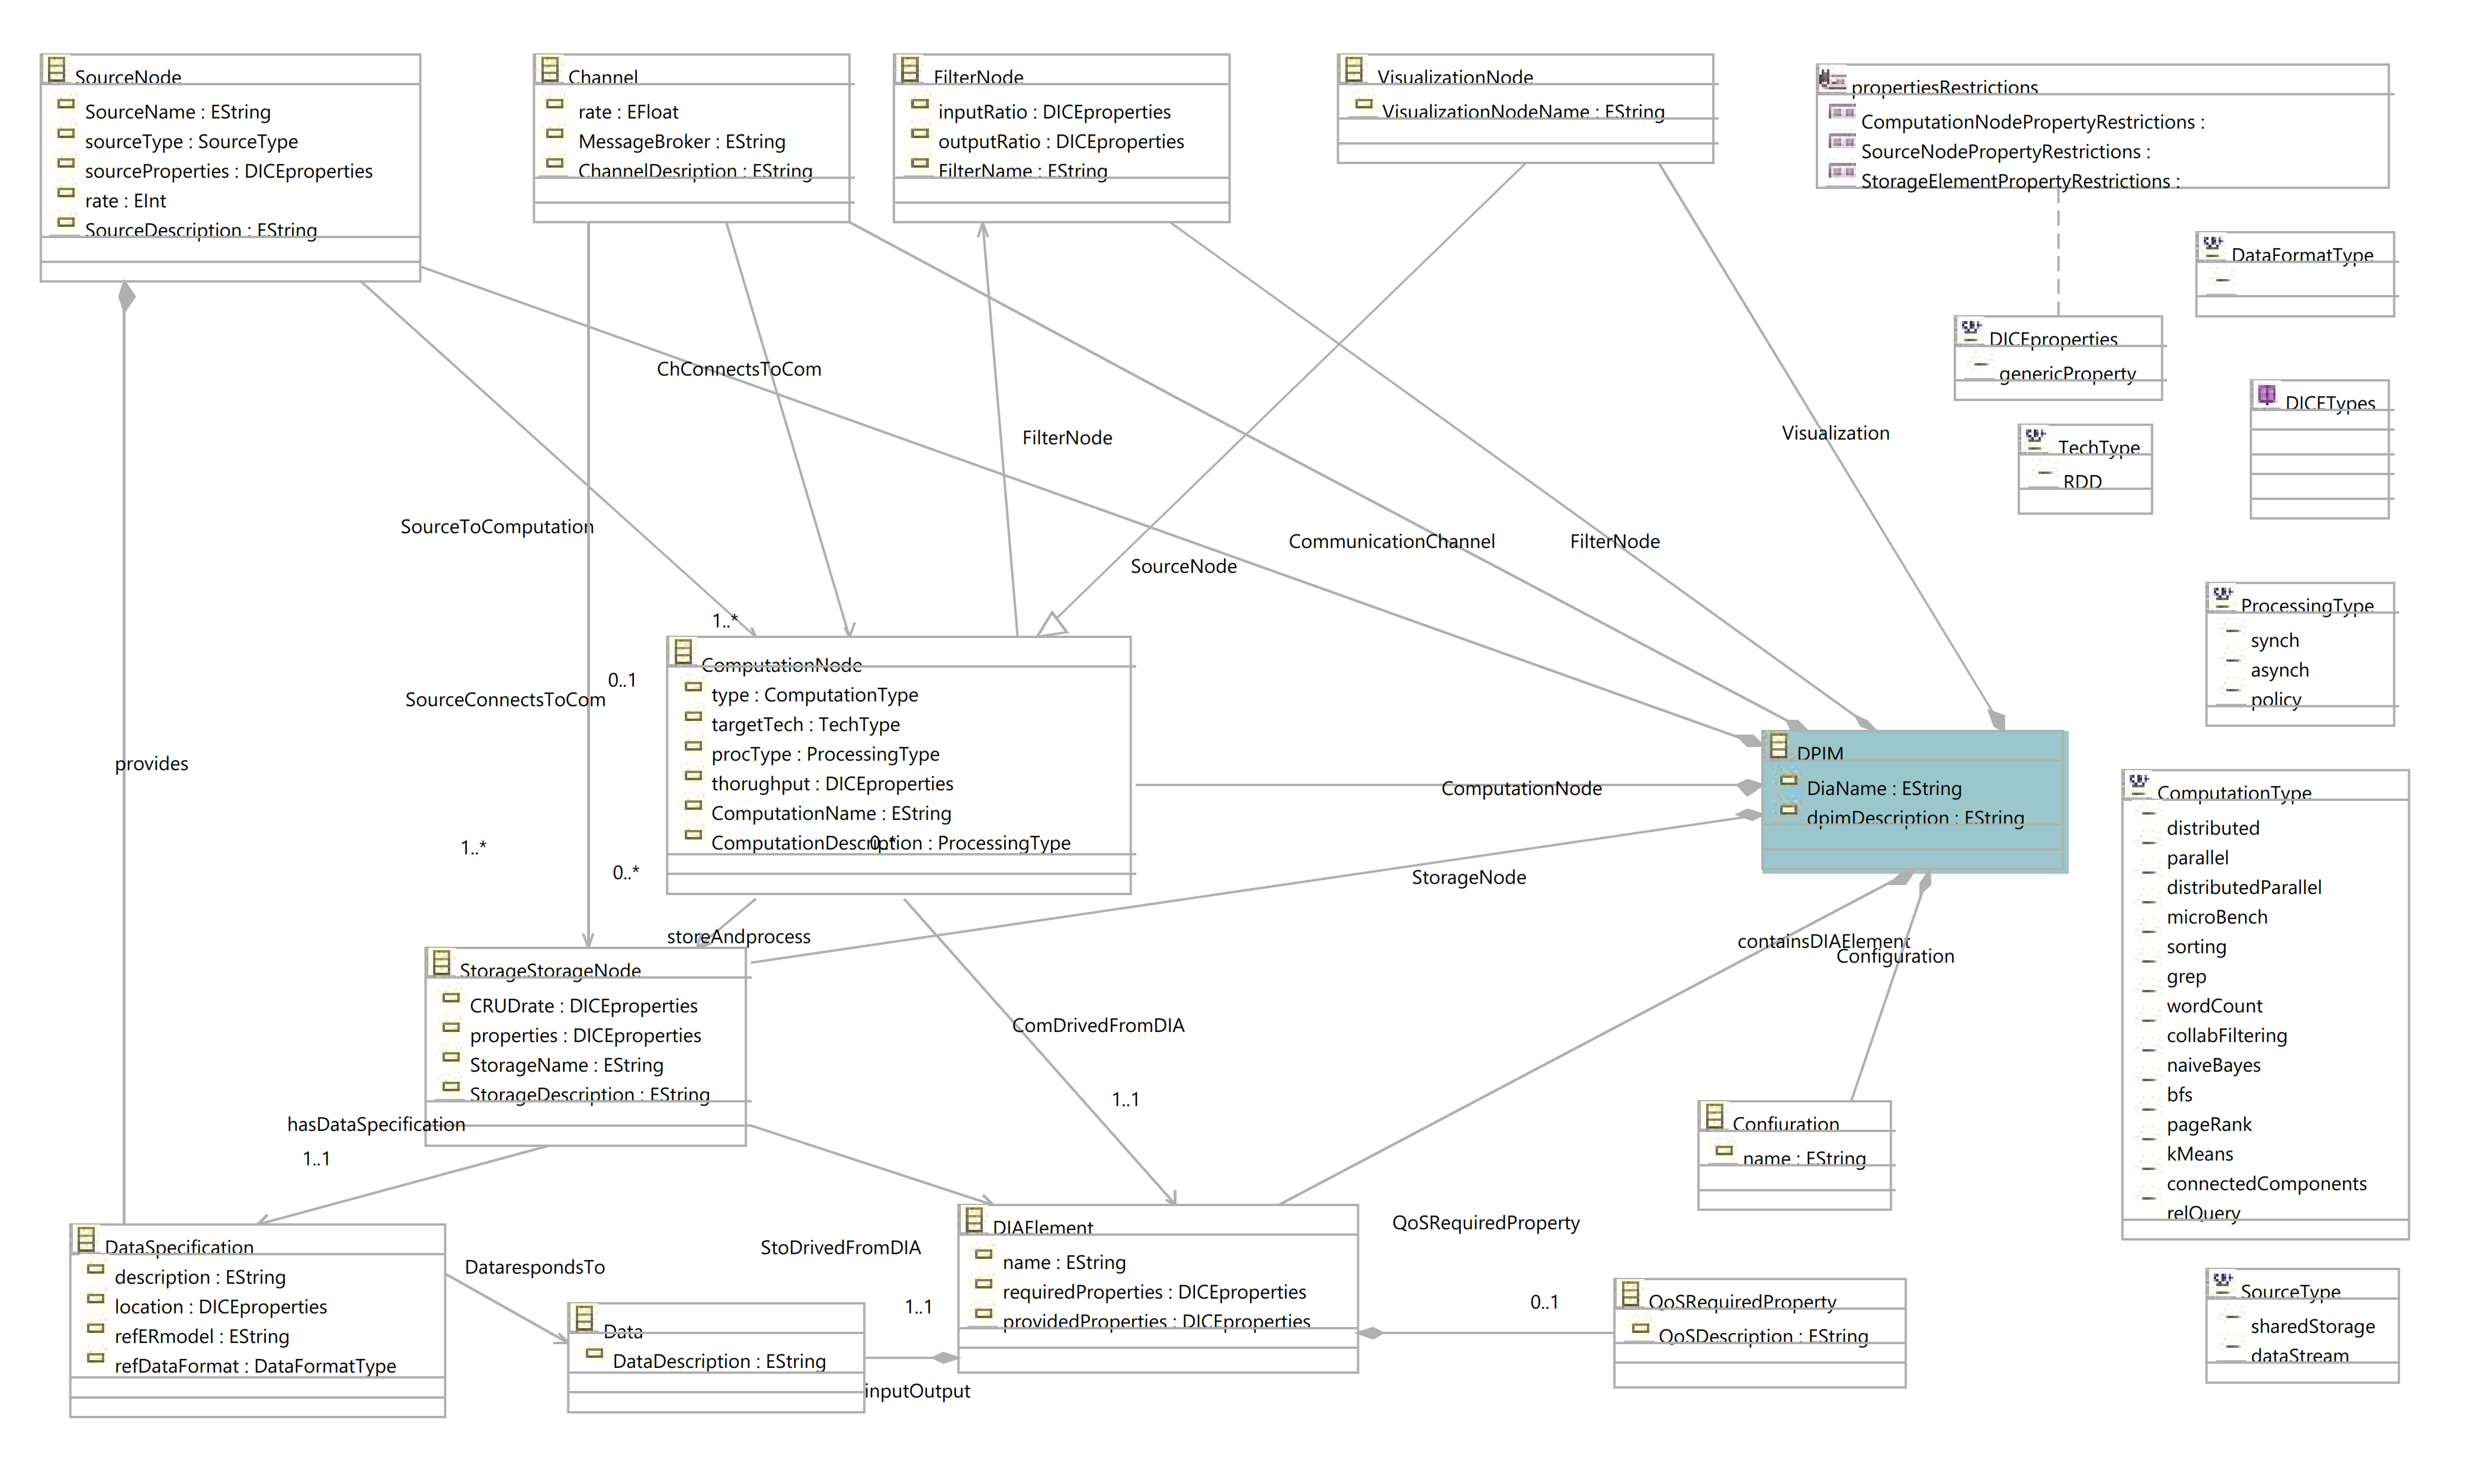
\includegraphics[width=\textwidth]{Images/11.png}
\caption{\label{fig:metamodel}DICE DPIM metamodel.}
\end{sidewaysfigure}

\begin{figure}
\centering
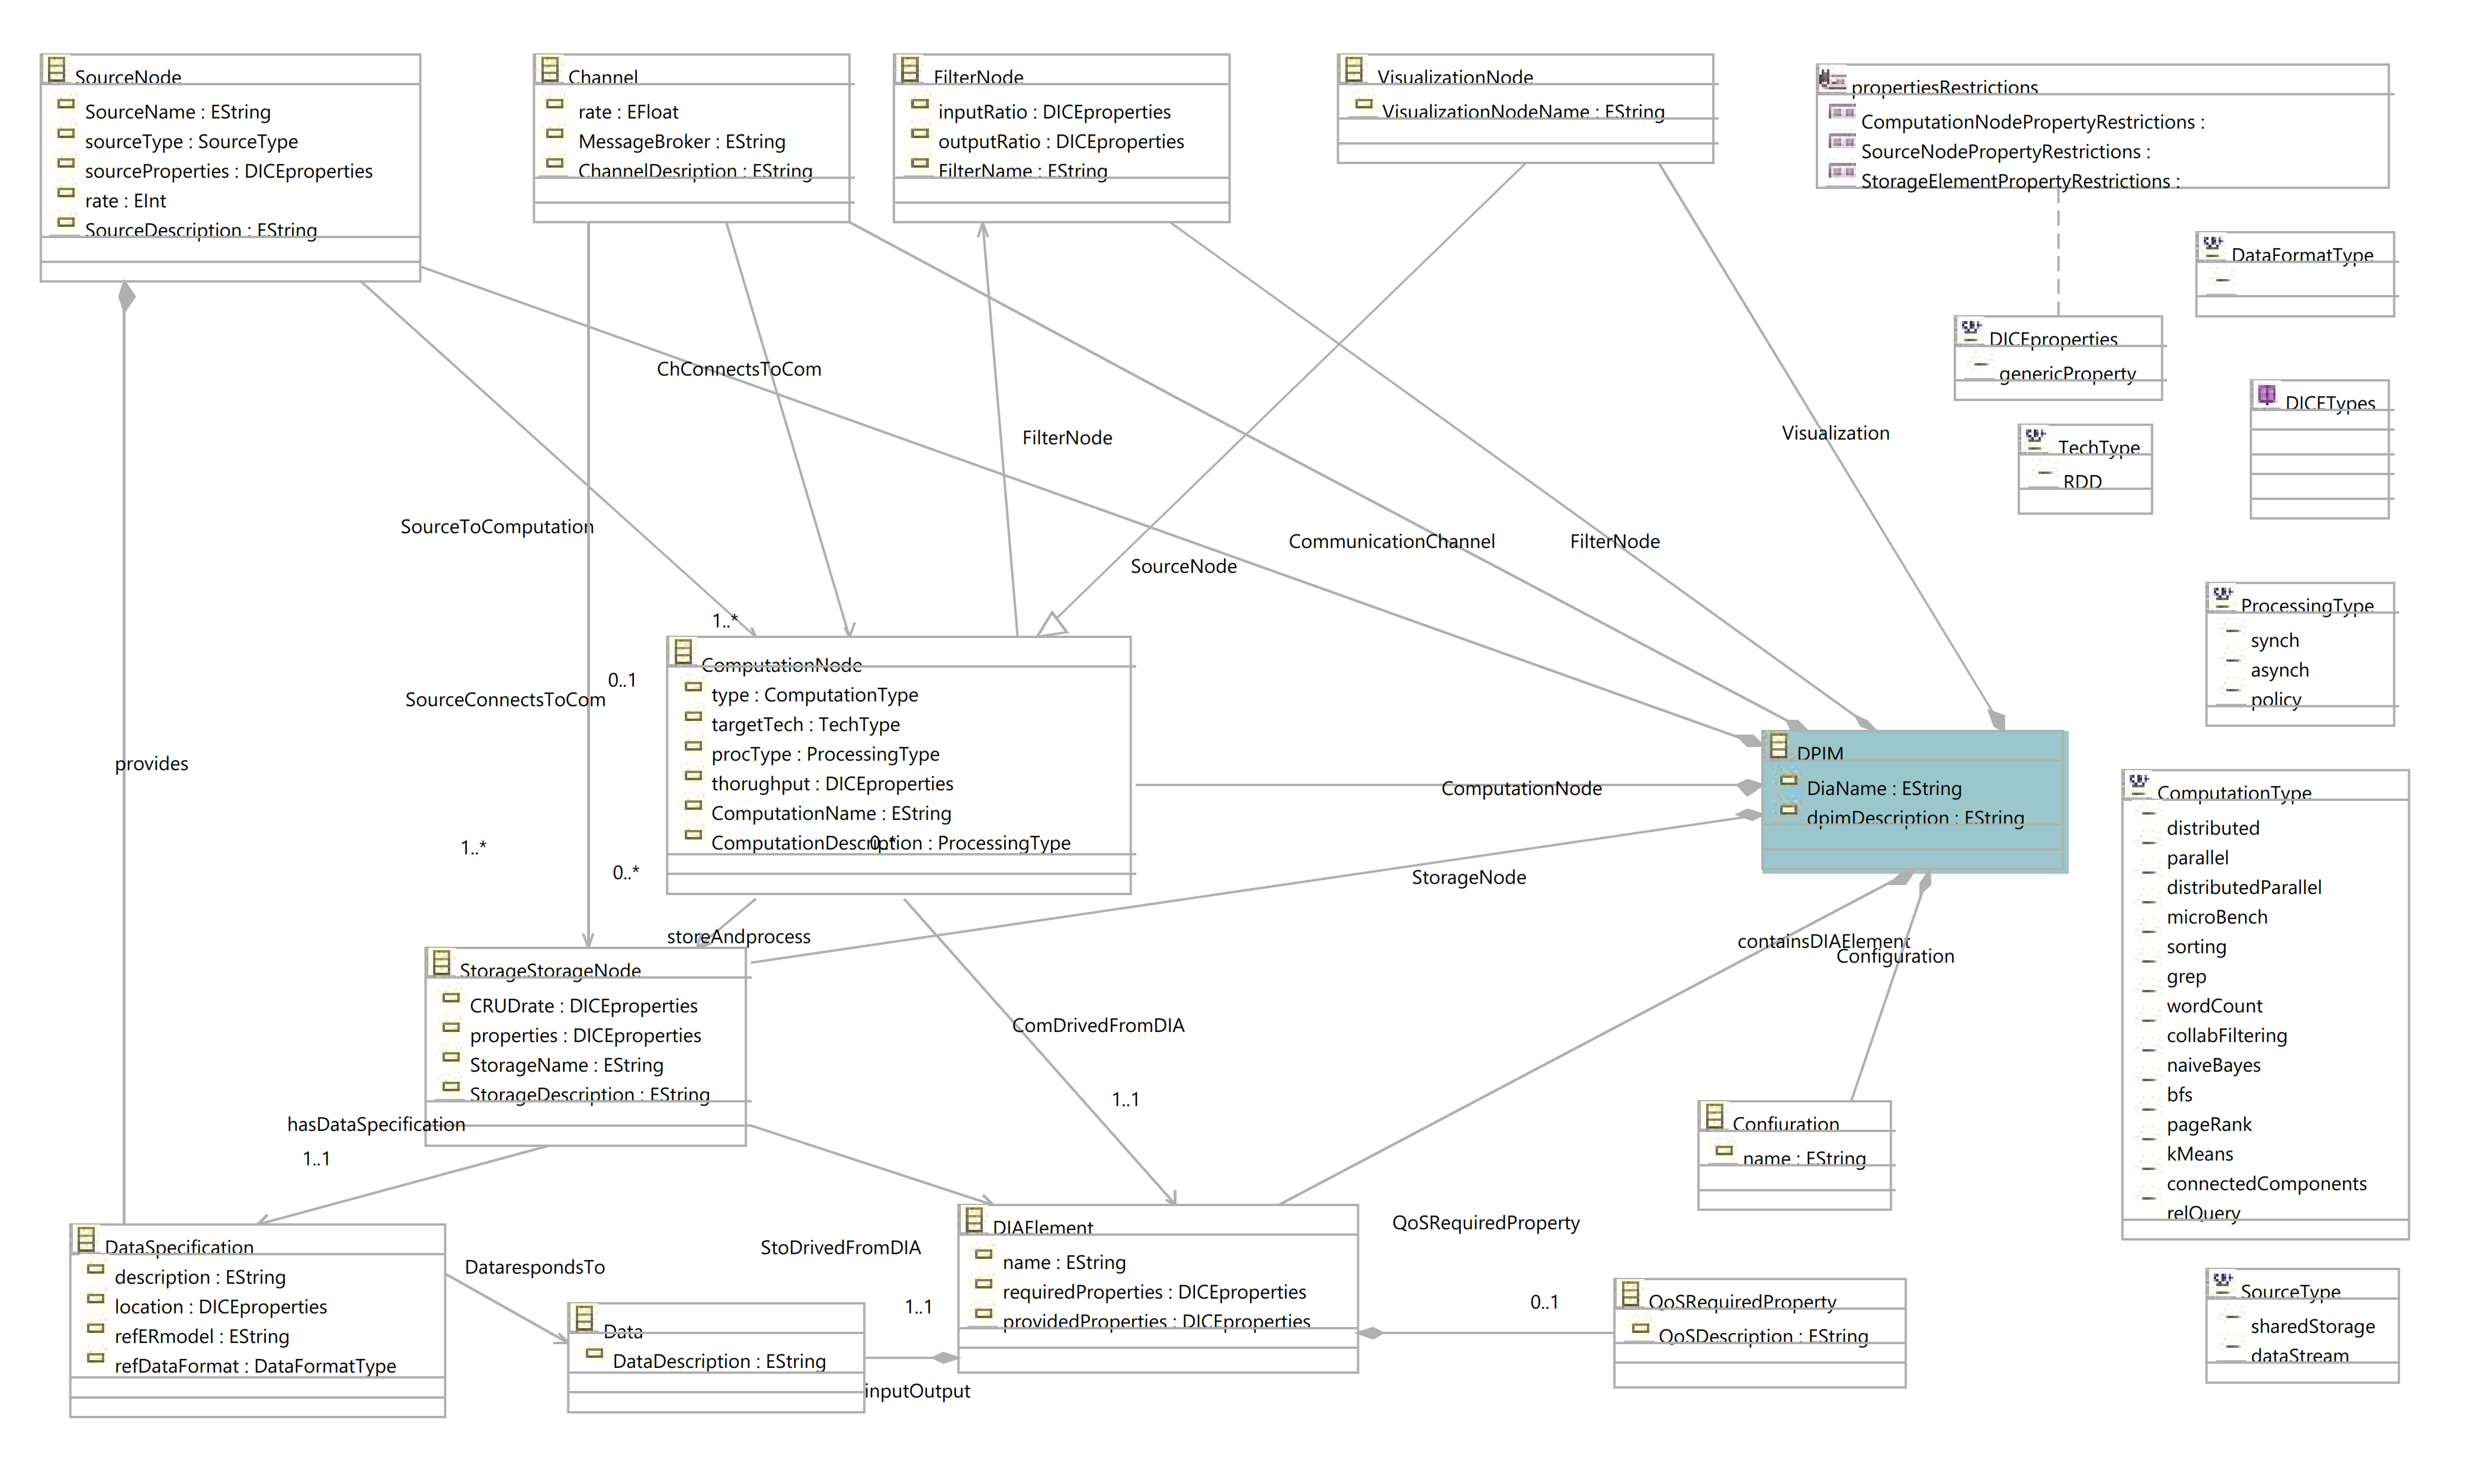
\includegraphics[width=\textwidth]{Images/11.png}
\caption{\label{fig:metamodel2}DICE DPIM metamodel in portrait form.}
\end{figure}

Here is the command to refer to another element (section, figure, table, ...) in the document: \emph{As discussed in Section~\ref{sect:overview} and as shown in Figure~\ref{fig:metamodel}, ...}. Here is how to introduce a bibliographic citation~\cite{DAM}. Bibliographic references should be included in a \texttt{.bib} file. 

Table generation is a bit complicated in Latex. You will soon become proficient, but to start you can rely on tools or external services. See for instance this \href{https://www.tablesgenerator.com}{https://www.tablesgenerator.com}. 


%------------------------------------------------------------------------------------------------------------------------------------------------
\clearpage
{\color{Blue}{\section{Specific Requirements}}}
\label{sect:requirements}
\subsection{External interface Requirements}
The \emph{CLup} frontend is a web application that can be accessed from web browsers, both from mobile and desktop devices. The following section will give a comprehensive description in terms of hardware, software and communication interfaces.

\subsubsection{Customer interfaces}
\textbf{Login and Registration}\\
\label{page:login}
When first opening the application, Customers are presented with a registration page. They are asked to provide only the essential information: an \emph{e-mail address} and a \emph{password}. The interface also shows a small button to switch to the login page, in case the customer has already signed in on another device or the session has expired. The page is identical to the one for the Registration, except for the Login button. In this case, the small button gives the Customers the ability to switch back to the registration page, which is needed if multiple people share the same device.
\begin{figure}[H]
    \centering
    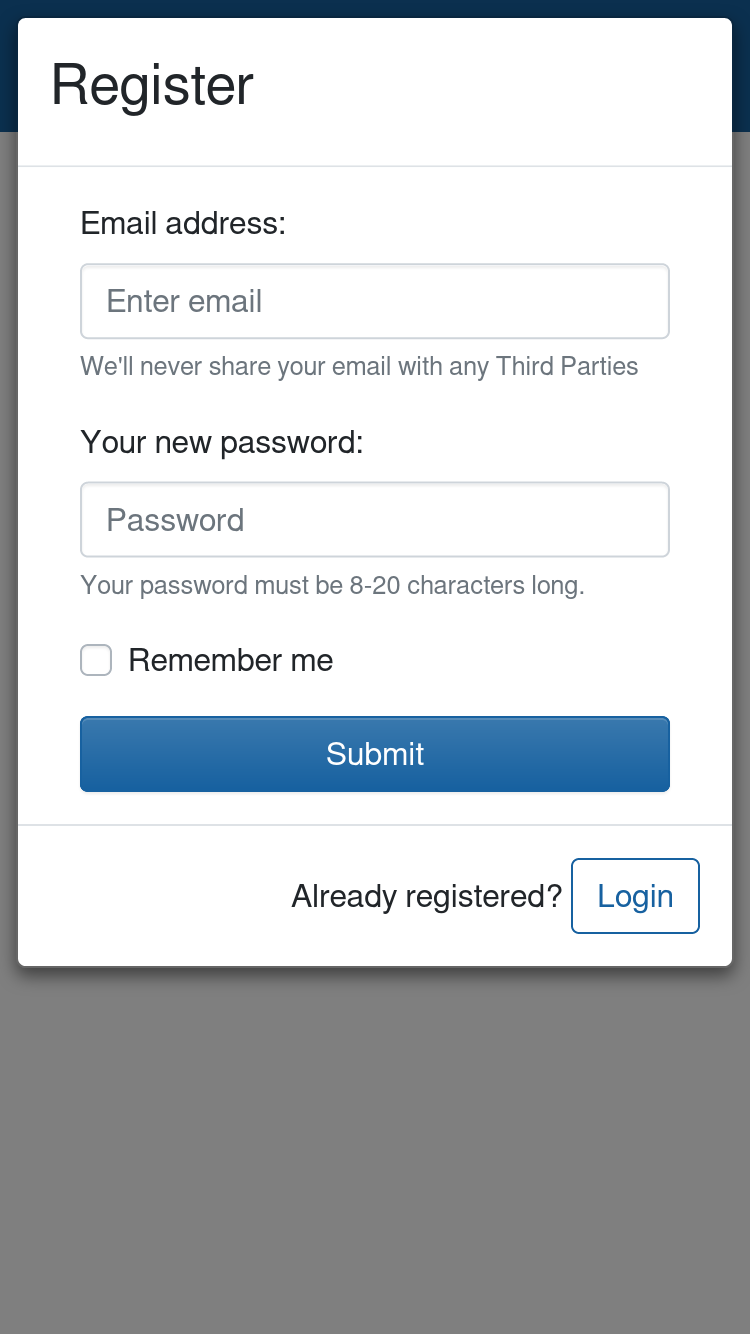
\includegraphics[scale=0.25]{Images/registration_mockup.png}
    \caption{Registration interface}
\end{figure}

% \begin{figure}[h]
%     \centering
%     \includegraphics[scale=0.63]{Images/login_register2.png}
%     \caption{Login interface}
% \end{figure}
\pagebreak
\textbf{Shop selection page}\\
\label{page:home}
After login/registration, the app displays a Shop search bar that dynamically updates its results while the Customers are typing. After selecting a Shop from the results, the two buttons "Get a Ticket" and "Make a Booking" are enabled, which are linked to the Ticket form and Booking form, respectively.
\begin{figure}[H]
    \begin{subfigure}{0.5\textwidth}
        \centering
        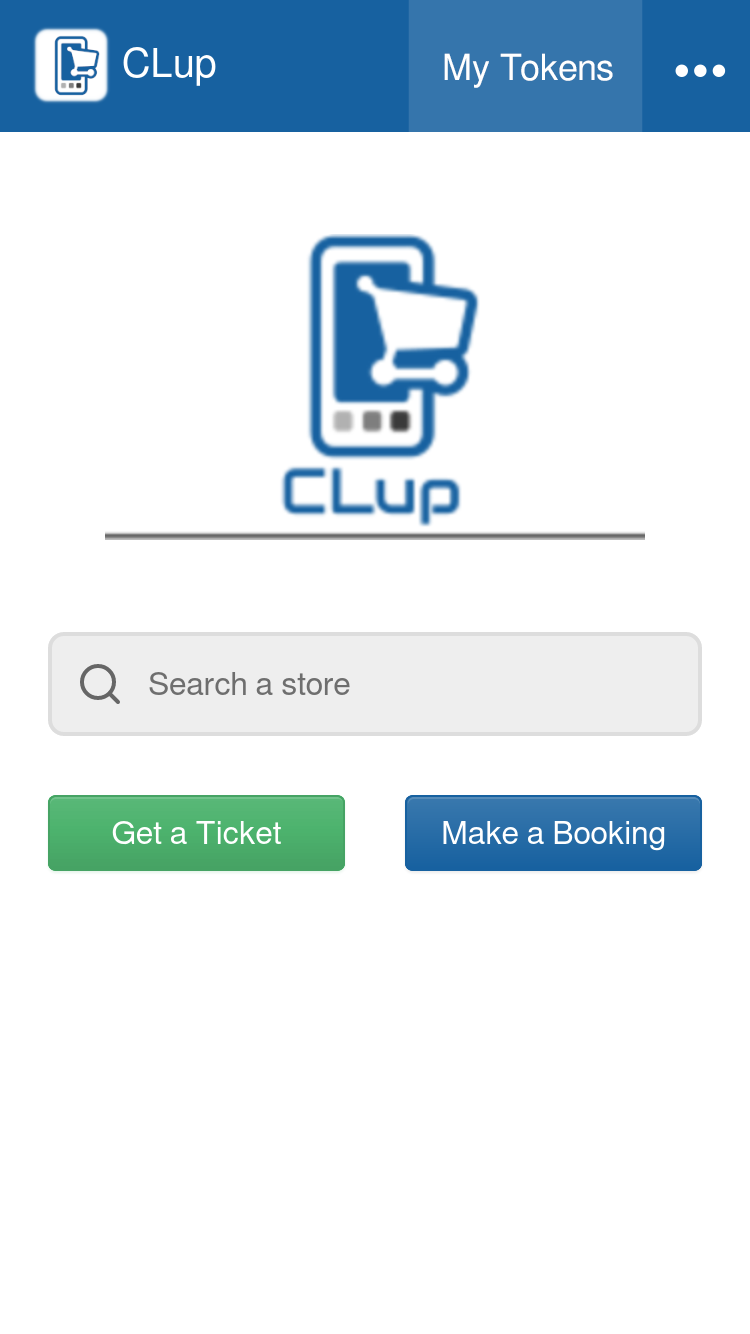
\includegraphics[width=0.75\textwidth]{Images/home-mockup.png}
        \caption{Shop selection interface}
    \end{subfigure}%
    \begin{subfigure}{0.5\textwidth}
        \centering
        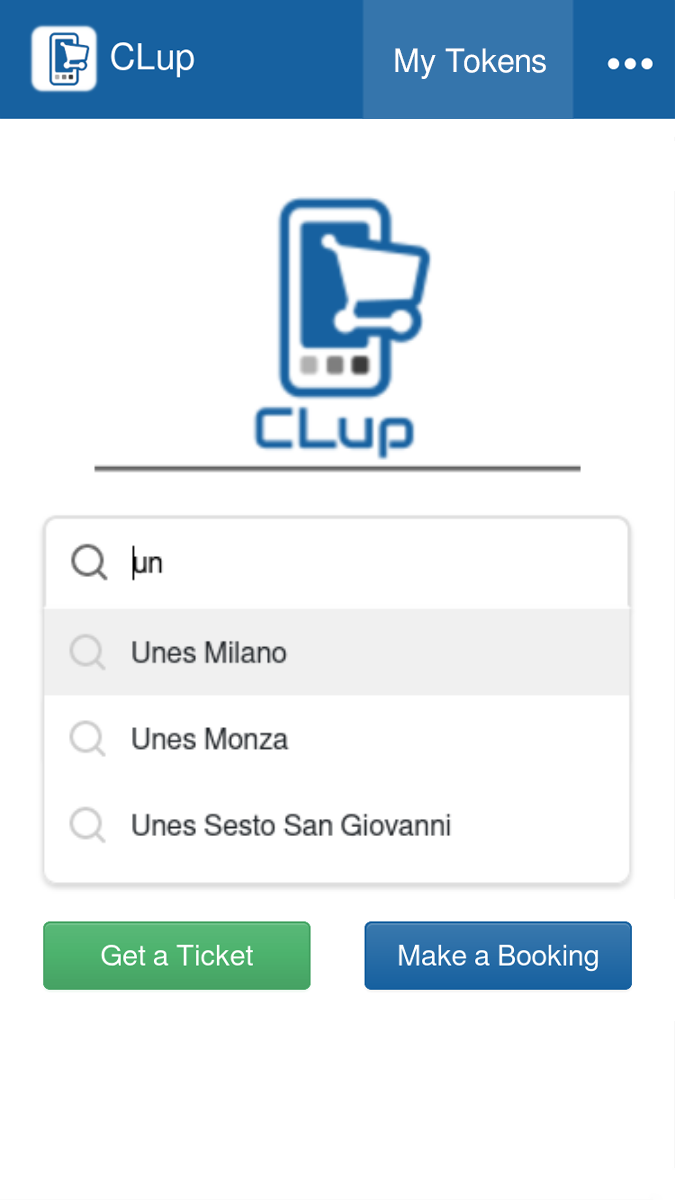
\includegraphics[width=0.75\textwidth]{Images/search-mockup.png}
        \caption{Dynamic search in the shop selection interface}
    \end{subfigure}
\end{figure}
\pagebreak
\textbf{Ticket form}\\
\label{page:ticket_form}
This page prompts Customers for an optional choice of categories they want to buy. Customers can confirm the Ticket request by pressing the \emph{"Submit"} button. In both the Ticket form and the Booking form, Customers are always given option to reset the app back to the Shop selection page.
\begin{figure}[H]
    \centering
    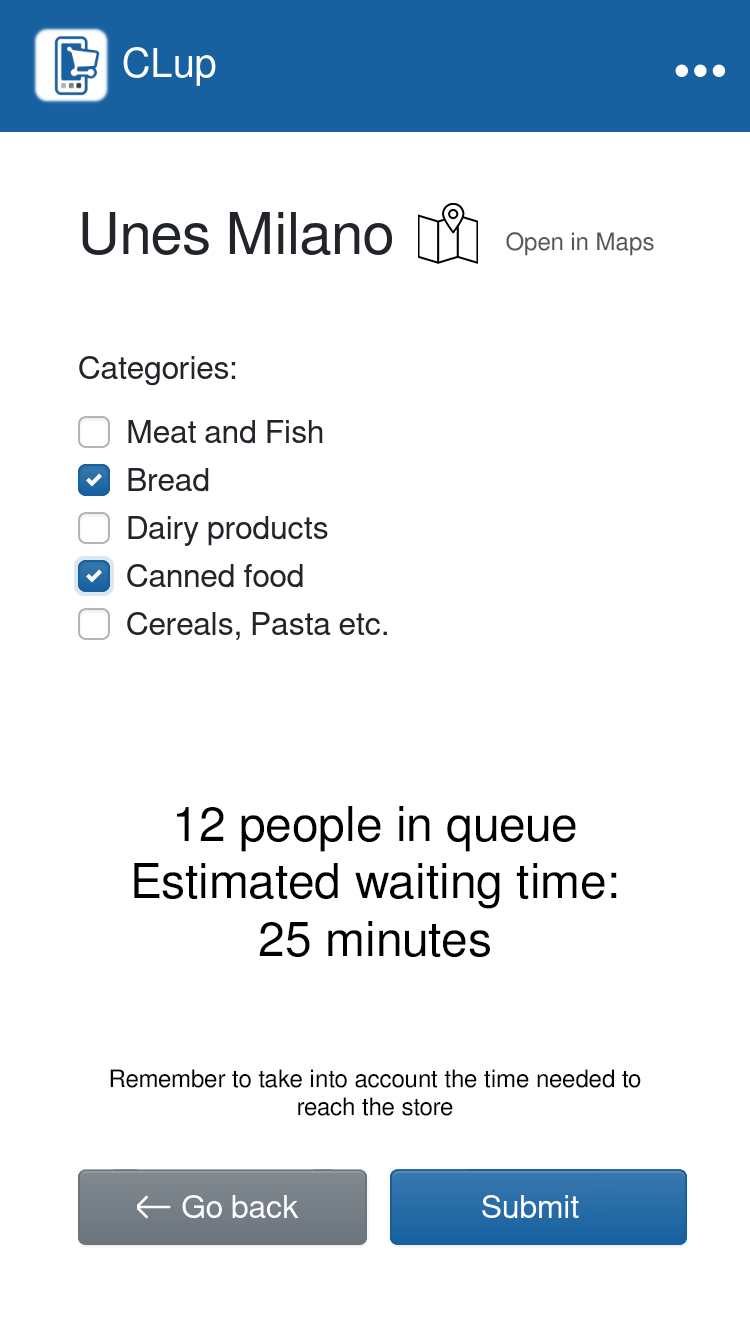
\includegraphics[scale=0.25]{Images/ticket-mockup.png}
    \caption{Ticket interface}
\end{figure}

\pagebreak
\textbf{Booking form}\\
\label{page:booking_form}
This page is identical to the previous, except for the added time selection. A table with days as columns and hours as rows shows the time slots with lower occupancy. When Customers select the preferred day, the visualization updates with specific data for the day, giving an in-depth visualization of restricted to the opening hours. Given this, Customers can easily choose a time for their visit. As in the Ticket form, Customers can confirm the Booking request by pressing the "Submit" button.
\begin{figure}[H]
    \centering
    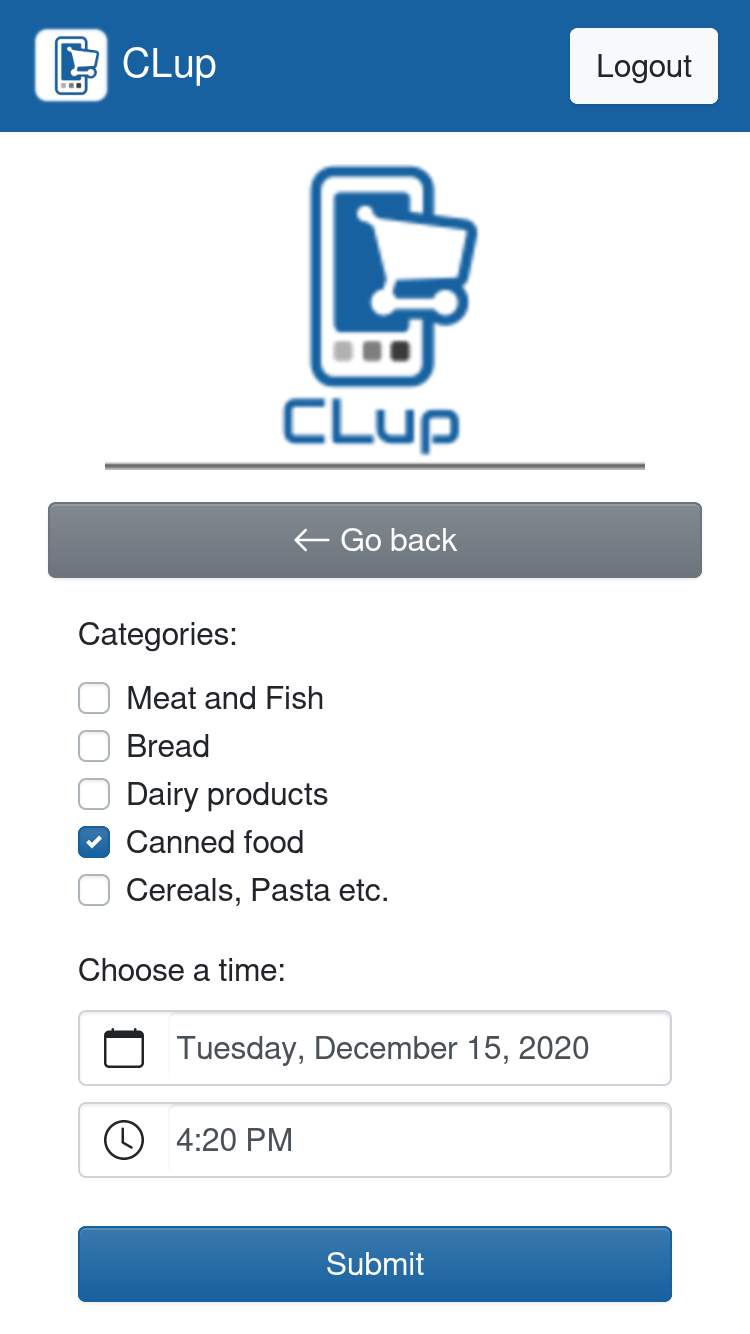
\includegraphics[scale=0.25]{Images/booking-mockup.png}
    \caption{Booking interface}
\end{figure}

\pagebreak
\textbf{Token display}\\
\label{page:token_show}
After generating a Ticket or a Booking, and until its expiration, the app will display the token as a fullscreen QR code right after opening, or after Login (if the login timeout has passed).
This makes it very quick to have the Token scanned by the clerks outside of a shop.
\begin{figure}[H]
    \begin{subfigure}{0.5\textwidth}
        \centering
        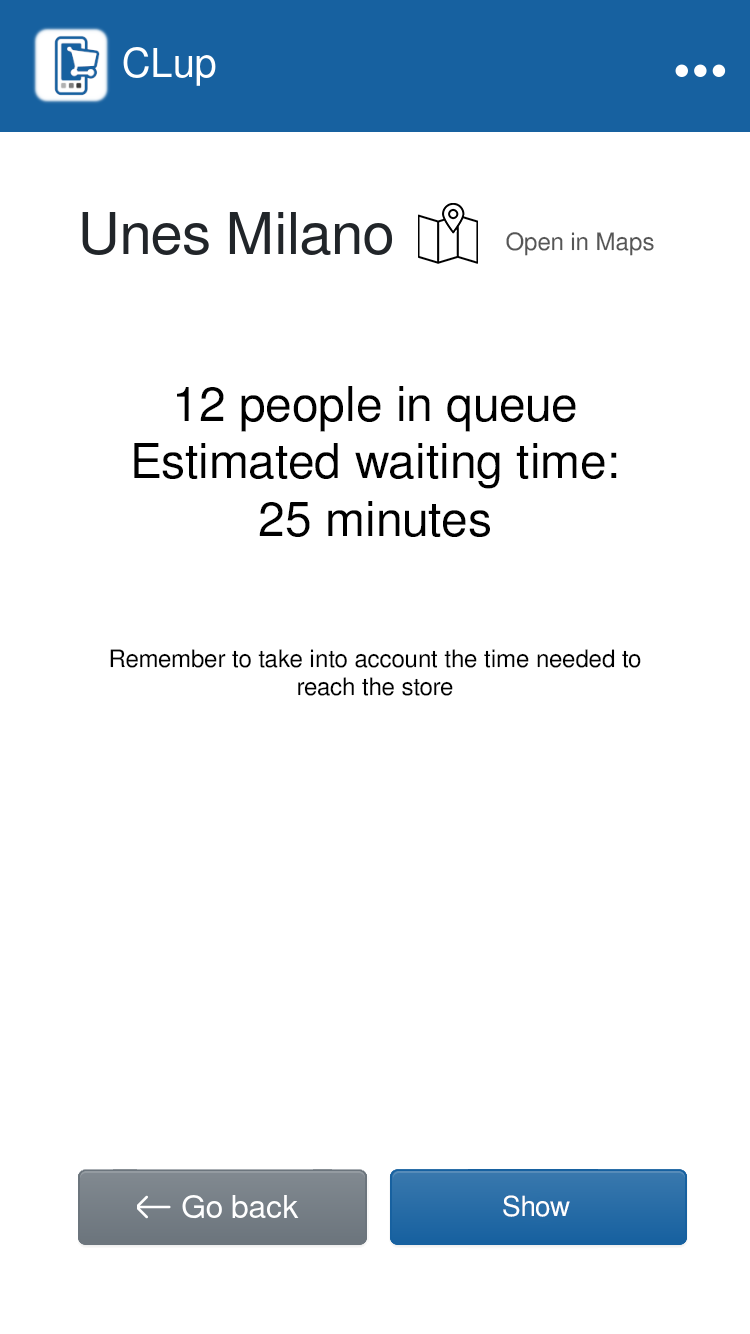
\includegraphics[width=0.75\textwidth]{Images/queue-mockup.png}
        \caption{My Tokens interface}
    \end{subfigure}%
    \begin{subfigure}{0.5\textwidth}
        \centering
        
\includegraphics[width=0.75\textwidth]{Images/token-mockup.png}
        \caption{Show token interface}
    \end{subfigure}
\end{figure}


\subsubsection{Hardware interfaces}
The \emph{CLup} client shall be available for devices capable of rendering a web page with javascript and internet access, this includes smartphones, tablets and personal computers.

Although not strictly required, the devices used by the staff should have a camera to scan QR codes

\subsubsection{Software interfaces}
\begin{itemize}
    \item \textbf{Web browser}: the applicative requires a web browser capable of rendering HTML5 web pages with Javascript
    \item \textbf{Maps service}: although not required for the core functionality, having access to a maps service on the device will improve customer experience
\end{itemize}

\subsubsection{Communication interfaces}
\begin{itemize}
    \item \emph{Customer}: requires a internet connection in order to get a token. Access to the store can be done offline if necessary.
    \item \emph{Staff}: requires a internet connection in order to communicate with the server and validate tokens or emit substitute tickets.
\end{itemize}
The system shall use the HTTPS protocol to provide secure communication from the client to the server.
\subsection{Functional requirements}

\subsubsection{Goal-Requirement mapping}
\begin{description}
    \item [G1] Customers shall be able to acquire a ticket which grants them access to the Shop
          \begin{description}
              \item [R1] The system shall keep track of the list of Customers waiting to visit each Shop
              \item [R2] The system shall allow customers to request the right to visit a shop as soon as possible
              \item [R3] The system shall give Customers a Token associated with their position in the waiting line
              \item [R4] The Staff shall be able to scan Customer generated Tokens using a camera
              \item [R5] The Staff shall be able to scan Customer generated Tokens using a textual input
              \item [R6] Given a Token, the Staff applicative shall be able to verify its validity
              \item [R7] Given a Token, the Staff applicative shall be able to verify the respective position in the waiting line
              \item [R8] Given a Token, the Staff applicative shall be able to mark it as used and update the list of Customers currently inside the Shop
          \end{description}
    \item [G2]  Customers shall be able to book a future visit to the Shop
          \begin{description}
              \item [R9] The system shall keep track of the Customers that want to visit a Shop in the future
              \item [R10] The system shall allow customers to choose a time in the future in which they wish ti visit a Shop
              \item [R11] The system shall give Customers a Token associated with their booking
              \item [R4] The Staff shall be able to scan Customer generated Tokens using a camera
              \item [R5] The Staff shall be able to scan Customer generated Tokens using a textual input
              \item [R6] Given a Token, the Staff applicative shall be able to verify its validity
              \item [R7] Given a Token, the Staff applicative shall be able to verify the respective position in the waiting line
              \item [R8] Given a Token, the Staff applicative shall be able to mark it as used and update the list of Customers currently inside the Shop
          \end{description}
    \item [G3]  Customers shall be able to enter the Shop at the earliest occasion without waiting in line
          \begin{description}
              \item [R1] The system shall keep track of the list of Customers waiting to visit each Shop
              \item [R9] The system shall keep track of the Customers that want to visit a Shop in the future
              \item [R12] The system shall ask Customers to specify the approximate duration of their visit
              \item [R13] The system shall automatically infer an estimate visit duration for returning customers
              \item [R14] The system shall give Customers an estimate of the waiting time remaining before it's their turn
              \item [R15] The system shall notify Customers when their turn is about to come
          \end{description}
    \item [G4]  Customers shall be reminded about considering the time needed to travel to the Shop
          \begin{description}
              \item [R14] The system shall give Customers an estimate of the waiting time remaining before it's their turn
              \item [R16] The system shall be able to connect to a Maps service to show information about travel time
          \end{description}
    \item [G5]  Third Parties shall better exploit the departments of the Shop without breaking social distancing measures
          \begin{description}
              \item [R17] Customers shall be able to specify the categories of items they intend to buy
              \item [R18] The system shall keep track of the number of customers visiting the Shop on a Department basis
          \end{description}
    \item [G6]  Third parties shall be able to monitor the number of visits to the Shop, to ensure compliance with the laws
          \begin{description}
              \item [R17] Customers shall be able to specify the categories of items they intend to buy
              \item [R18] The system shall keep track of the number of customers visiting the Shop on a Department basis
          \end{description}
\end{description}

\subsubsection{Scenarios}
\textbf{Scenario 1}\\
Maria is gathering ingredients to bake a cake, but she realizes she doesn't have any milk.
Maria lives near to a grocery shop so she opens the web app, she writes the shop name in the search bar and she is presented with the most relevant matches. She clicks on the shop and then she chooses \emph{"Get a Ticket"}. Now she checks the dairy section and confirms, receiving her ticket.
CLup shows that Maria's turn will be in about 10 minutes. Five minutes later she checks back on the app and the approximate time is now 5 minutes, so she leaves and she goes to the shop.
At the shop Giovanni, a memeber of the staff, is at the entrance waiting for customers. Maria is welcomed by Giovanni, she opens the application and she shows him the ticket, Giovanni scans the ticket with his phone, Maria is just in time, so she can enter the shop and do her groceries.
At the exit she is invited by Mario, another member of the staff to scan her ticket, she shows the ticket one last time, then she leaves the shop and returns home ready to bake a cake.

\textbf{Scenario 2}\\
Marco has a busy schedule for the week and he needs to go and get a suit for an important meeting. He looks at his schedule and finds a spot on thursday, so he opens the web app, he writes the shop name in the search bar and she is presented with the most relevant matches. He clicks on the shop and then he chooses \emph{"Make a Booking"}. Then he checks the clothing section and clicks on thursday on the calendar luckily there is a free time slot. So he inputs the time and confirms, the app responds with the token for the booking. On thursday Marco goes to the shop in time for his booking, he is welcomed by Francesca, a staff member, and shows her the QR code associated with his booking, she scans it using her phone and Marco is allowed in. At the exit he is invited to scan his booking one last time before leaving.

\textbf{Scenario 3}\\
Attilio was never a fan of technology and he does not have a smartphone, unfortuanately his grandchild Matteo is not around to get a ticket for him, so he picks up his bicycle and goes to the grocery shop. At the entrance to the shop Francesco, a staff member, informs Attilio about the new procedure to enter the shop, since Attilio does not have a smartphone Fancesco uses his device to create a substitute ticket and prints it. Francesco hands Attilio the ticket, then he tells him that there are already 5 people waiting, so he will have to wait for about 10 minutes. Ten minutes later Attilio goes back to the entrance where Francesco scans the ticket letting Attilio go in. At the exit he is invited to scan the ticket one last time before heading home.

\subsubsection{Use cases}

\begin{figure}[H]
    \centering
    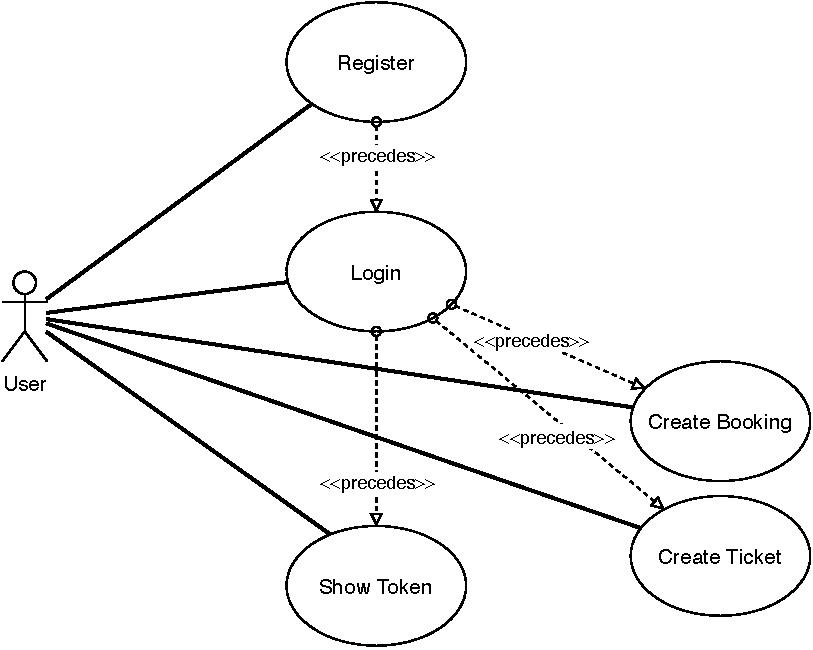
\includegraphics[width=0.7\textwidth]{Images/usecasediagram-user.pdf}
    \caption{Use Case Diagram: Customer}
\end{figure}
\begin{figure}[H]
    \centering
    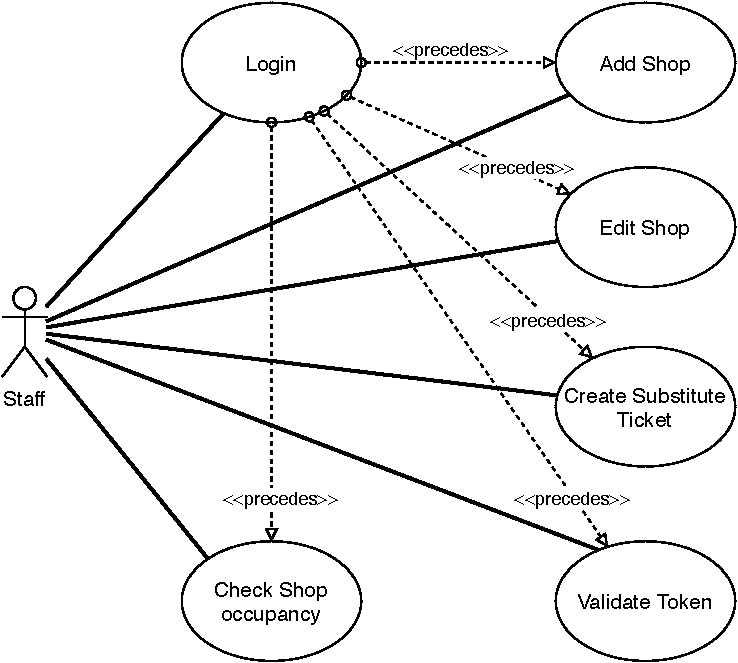
\includegraphics[width=0.7\textwidth]{Images/usecasediagram-staff.pdf}
    \caption{Use Case Diagram: Authority}
\end{figure}

\begin{table}[H]
    \begin{tabu} to \textwidth {|X|X[4]|}
        \hline
        Name            & Customer creates an account \\ \hline
        Actor           & Customer                    \\ \hline
        Entry condition & \begin{itemize}
            \item The Customer has not created an account yet
        \end{itemize}  \\ \hline
        Event flow      & \begin{enumerate}
            \item The Customer opens the web app
            \item The app asks for login or registration
            \item The Customer clicks on \emph{"Register"}
            \item The Customer inserts their email and password
            \item The Customer clicks on \emph{"Submit"}
            \item The app prompts the Customer to check their email for a confirmation link
            \item The Customer clicks on the confirmation link
        \end{enumerate}  \\ \hline
        Exit condition  & \begin{itemize}
            \item Customer account is added to the database
            \item The Customer can login
        \end{itemize}  \\ \hline
        Exceptions      & \begin{itemize}
            \item The Customer already exists
            \item The Customer does not click confirmation link
        \end{itemize}  \\ \hline
    \end{tabu}
\end{table}

\begin{table}[H]
    \begin{tabu} to \textwidth {|X|X[4]|}
        \hline
        Name            & Customer logs in           \\ \hline
        Actor           & Registered Customer        \\ \hline
        Entry condition & \begin{itemize}
            \item The Customer has an account
        \end{itemize} \\ \hline
        Event flow      & \begin{enumerate}
            \item The Customer opens the web app
            \item The app asks for login or registration
            \item The Customer inserts their email and password
            \item The Customer clicks on \emph{"Submit"}
            \item The Customer receives confirmation from the server
            \item The Customer is brought to the home page
        \end{enumerate} \\ \hline
        Exit condition  & \begin{itemize}
            \item The Customer is logged in
            \item The Customer can use other features
        \end{itemize} \\ \hline
        Exceptions      & \begin{itemize}
            \item Wrong credentials
        \end{itemize} \\ \hline
    \end{tabu}
\end{table}

\begin{table}[H]
    \begin{tabu} to \textwidth {|X|X[4]|}
        \hline
        Name            & Customer creates a booking \\ \hline
        Actor           & Customer                   \\ \hline
        Entry condition & \begin{itemize}
            \item The Customer has logged in
        \end{itemize} \\ \hline
        Event flow      & \begin{enumerate}
            \item The Customer types all or part of the shop name in the search bar
            \item Results are dynamically updated
            \item The Customer selects one of the results
            \item The Customer clicks on \emph{"Make a booking"}
            \item The Customer is brought to the \emph{Booking form}
            \item The Customer chooses a day from the calendar
            \item The Customer inputs the desired time of visit
            \item The Customer can choose the departments it will visit
            \item The Customer clicks submit
            \item The Customer receives confirmation from the server and is shown the new booking
        \end{enumerate} \\ \hline
        Exit condition  & \begin{itemize}
            \item Booking is added to the database
            \item The Customer can now find the new token in his tokens
        \end{itemize} \\ \hline
        Exceptions      & \begin{itemize}
            \item Shop does not exist
            \item Shop is already completely booked
            \item The Customer tries to book an already full time slot
        \end{itemize} \\ \hline
    \end{tabu}
\end{table}

\begin{table}[H]
    \begin{tabu} to \textwidth {|X|X[4]|}
        \hline
        Name            & Customer creates a ticket  \\ \hline
        Actor           & Customer                   \\ \hline
        Entry condition & \begin{itemize}
            \item The Customer has logged in
        \end{itemize} \\ \hline
        Event flow      & \begin{enumerate}
            \item The Customer types all or part of the shop name in the search bar
            \item Results are dynamically updated
            \item The Customer selects one of the results
            \item The Customer clicks on \emph{"Get a Ticket"}
            \item The Customer is brought to the \emph{Get ticket form}
            \item The Customer clicks submit
            \item The Customer receives confirmation from the server and is shown the new ticket
        \end{enumerate} \\ \hline
        Exit condition  & \begin{itemize}
            \item Ticket is added to the database
            \item The Customer can now find the new token in his tokens
        \end{itemize} \\ \hline
        Exceptions      & \begin{itemize}
            \item Shop does not exist
            \item Shop is closed for the day
            \item Shop queue is full
        \end{itemize} \\ \hline
    \end{tabu}
\end{table}

\begin{table}[H]
    \begin{tabu} to \textwidth {|X|X[4]|}
        \hline
        Name            & Customer shows a token     \\ \hline
        Actor           & Customer                   \\ \hline
        Entry condition & \begin{itemize}
            \item The Customer has logged in
            \item The Customer has created at least one token
        \end{itemize} \\ \hline
        Event flow      & \begin{enumerate}
            \item The Customer clicks on \emph{"My Tokens"}
            \item The Customer selects one of the tokens in the list
            \item A QR code and associated text code are shown, either of which can be scanned with the staff applicative
        \end{enumerate} \\ \hline
    \end{tabu}
\end{table}

\begin{table}[H]
    \begin{tabu} to \textwidth {|X|X[4]|}
        \hline
        Name            & Manager adds a shop        \\ \hline
        Actor           & Staff                      \\ \hline
        Entry condition & \begin{itemize}
            \item The Manager is logged in with an administrative account
        \end{itemize} \\ \hline
        Event flow      & \begin{enumerate}
            \item The Manager opens the "Manage Shops" section
            \item The Manager clicks on add a Shop
            \item The Manager inserts the Shop name and location
            \item The Manager adds departments to the Shop and specifies the max capacity of each
            \item The Manager specifies the opening hours
            \item The Manager clicks on submit
            \item The Manager receives confirmation from the server
        \end{enumerate} \\ \hline
        Exit condition  & \begin{itemize}
            \item The new Shop is added to the database
            \item Customers can find the Shop in hteir search results
        \end{itemize} \\ \hline
        Exceptions      & \begin{itemize}
            \item The Shop already exists
        \end{itemize} \\ \hline
    \end{tabu}
\end{table}

\begin{table}[H]
    \begin{tabu} to \textwidth {|X|X[4]|}
        \hline
        Name            & Staff scans a valid token  \\ \hline
        Actor           & Staff                      \\ \hline
        Entry condition & \begin{itemize}
            \item The Staff member is Logged in
            \item The Staff member selected one of the shops they have access to
            \item A Customer shows a token that is valid at the current time
        \end{itemize} \\ \hline
        Event flow      & \begin{enumerate}
            \item The Staff member opens the scan token section
            \item The Staff member uses the camera of the device to scan the token from an Customer or inputs the code as text
            \item The token is sent to the server for validation
            \item The Staff member receives positive confirmation from the server
            \item The Customer is allowed in
        \end{enumerate} \\ \hline
        Exit condition  & \begin{itemize}
            \item The token is marked as used
            \item The store occupancy statistics are updated
        \end{itemize} \\ \hline
        Exceptions      & \begin{itemize}
            \item The token is for another shop
        \end{itemize} \\ \hline
    \end{tabu}
\end{table}

\begin{table}[H]
    \begin{tabu} to \textwidth {|X|X[4]|}
        \hline
        Name            & Staff scans an invalid token \\ \hline
        Actor           & Staff                        \\ \hline
        Entry condition & \begin{itemize}
            \item The Staff member is Logged in
            \item The Staff member selected one of the shops they have access to
            \item A Customer shows a token which is either expired or not yet valid
        \end{itemize}   \\ \hline
        Event flow      & \begin{enumerate}
            \item The Staff member opens the scan token section
            \item The Staff member uses the camera of the device to scan the token from an Customer or inputs the code as text
            \item The token is sent to the server for validation
            \item The Staff member receives a negative response from the server
            \item The Customer informed that either their ticket is expired or that it's too early
            \item The Customer is not allowed in
        \end{enumerate}   \\ \hline
        Exit condition  & \begin{itemize}
            \item The token is marked as used
            \item The store occupancy statistics are updated
        \end{itemize}   \\ \hline
        Exceptions      & \begin{itemize}
            \item The token is for another shop
        \end{itemize}   \\ \hline
    \end{tabu}
\end{table}

\begin{table}[H]
    \begin{tabu} to \textwidth {|X|X[4]|}
        \hline
        Name            & Staff creates a substitute ticket \\ \hline
        Actor           & Staff                             \\ \hline
        Entry condition & \begin{itemize}
            \item The Staff member is Logged in
            \item The Staff member selected one of the shops they have access to
            \item A Customer without the applicative asks for a ticket
        \end{itemize}        \\ \hline
        Event flow      & \begin{enumerate}
            \item The Staff member opens the create substitute ticket section
            \item The Staff member asks the Customer and inputs the departments they wish to visit
            \item The Staff member clicks on submit
            \item The Staff member prints the token and hands it to the Customer
            \item The Staff member reads the esimated wait time to the Customer
        \end{enumerate}        \\ \hline
        Exit condition  & \begin{itemize}
            \item The substitute ticket is added to the database
            \item The Customer can use the token to access the Shop when it's their turn in the queue
        \end{itemize}        \\ \hline
        Exceptions      & \begin{itemize}
            \item The queue is full
        \end{itemize}        \\ \hline
    \end{tabu}
\end{table}

\begin{table}[H]
    \begin{tabu} to \textwidth {|X|X[4]|}
        \hline
        Name            & Manager checks shop occupancy \\ \hline
        Actor           & Staff                         \\ \hline
        Entry condition & \begin{itemize}
            \item The Manager is Logged in with an administrative account
        \end{itemize}    \\ \hline
        Event flow      & \begin{enumerate}
            \item The Manager selects a Shop from those available
            \item The system shows the available occupancy statistcs
        \end{enumerate}    \\ \hline
        Exceptions      & \begin{itemize}
            \item The Manager does not have any listed shop
        \end{itemize}    \\ \hline
    \end{tabu}
\end{table}

\subsubsection{Sequence diagrams}
\begin{figure}[H]
    \centering
    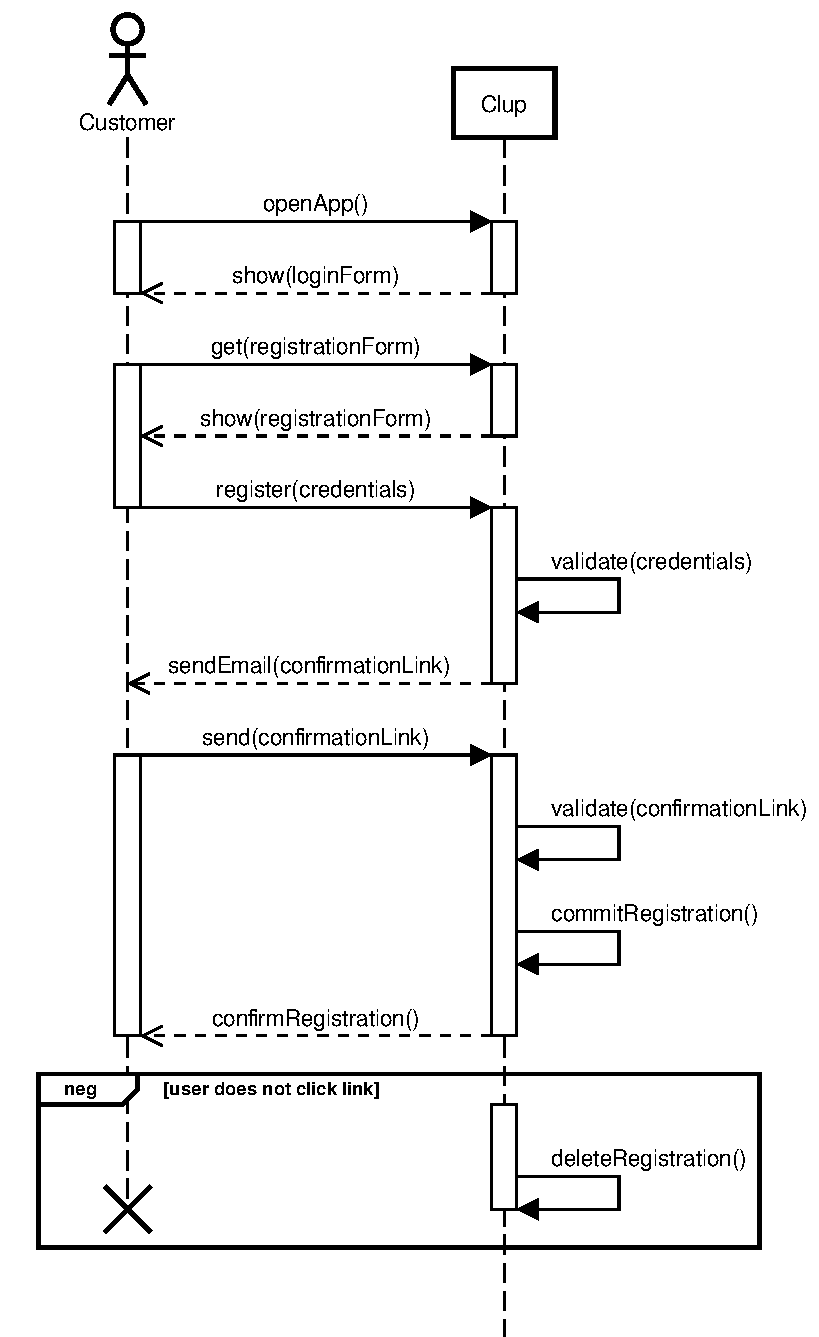
\includegraphics[scale=0.9]{Images/Sequence/create-account_sequence_straight.pdf}
    \caption{Sequence Diagram for the registration of a Customer}
\end{figure}
\begin{figure}[H]
    \centering
    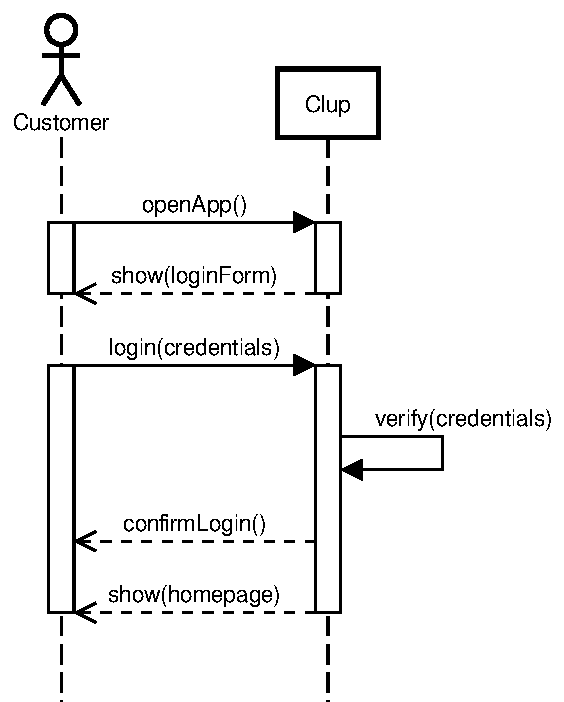
\includegraphics[scale=0.9]{Images/Sequence/login-account_sequence_straight.pdf}
    \caption{Sequence Diagram for a successful login attempt}
\end{figure}
\begin{figure}[H]
    \centering
    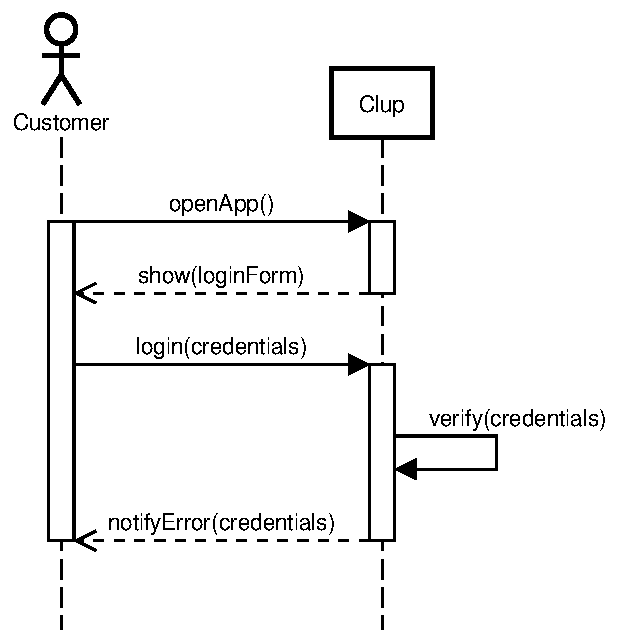
\includegraphics[scale=0.9]{Images/Sequence/failedlogin-account_sequence_straight.pdf}
    \caption{Sequence Diagram for a failed login attempt}
\end{figure}
\begin{figure}[H]
    \centering
    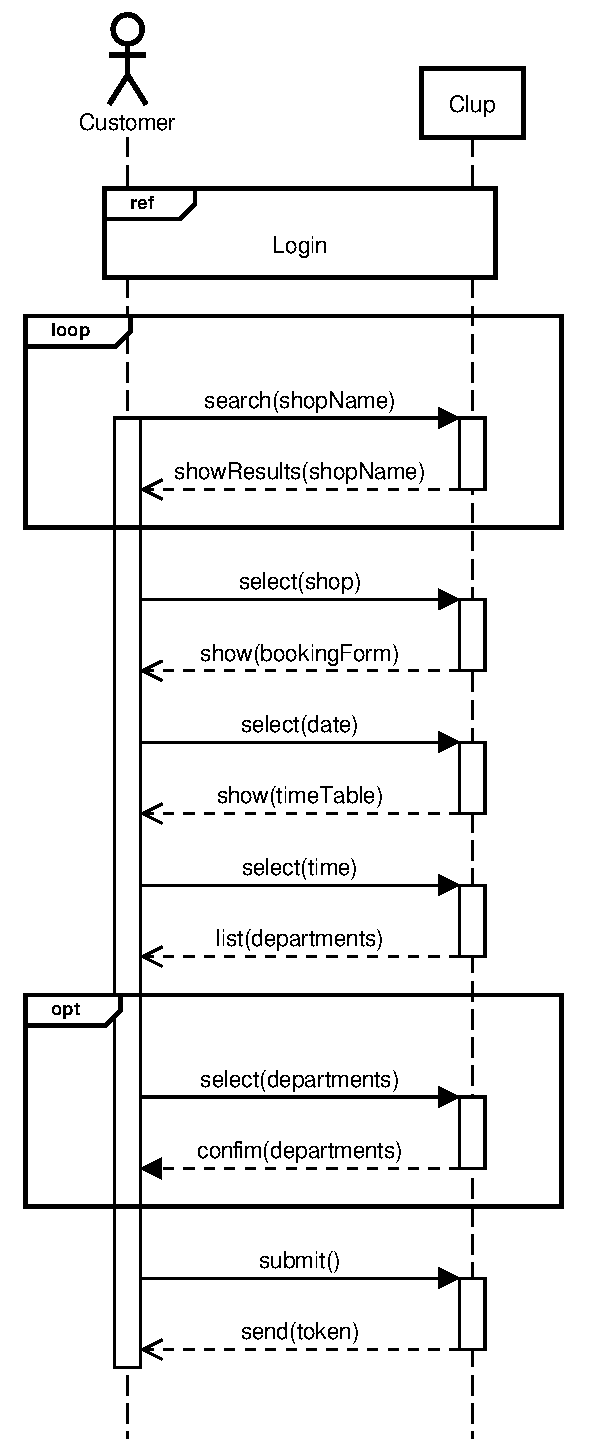
\includegraphics[scale=0.9]{Images/Sequence/booking-loop_sequence_straight.pdf}
    \caption{Sequence Diagram for the creation of a Booking}
\end{figure}
\begin{figure}[H]
    \centering
    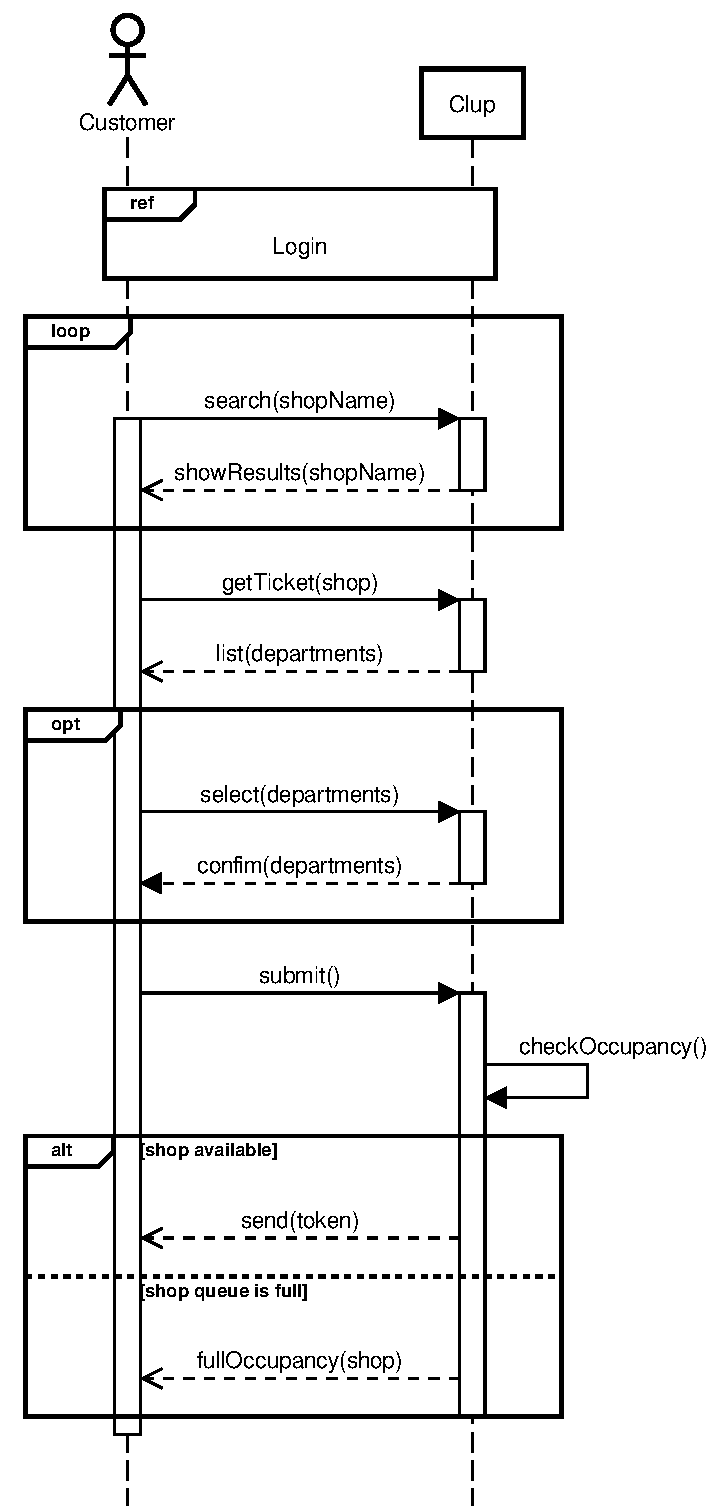
\includegraphics[scale=0.9]{Images/Sequence/ticket_sequence_straight.pdf}
    \caption{Sequence Diagram for the creation of a Ticket}
\end{figure}
\begin{figure}[H]
    \centering
    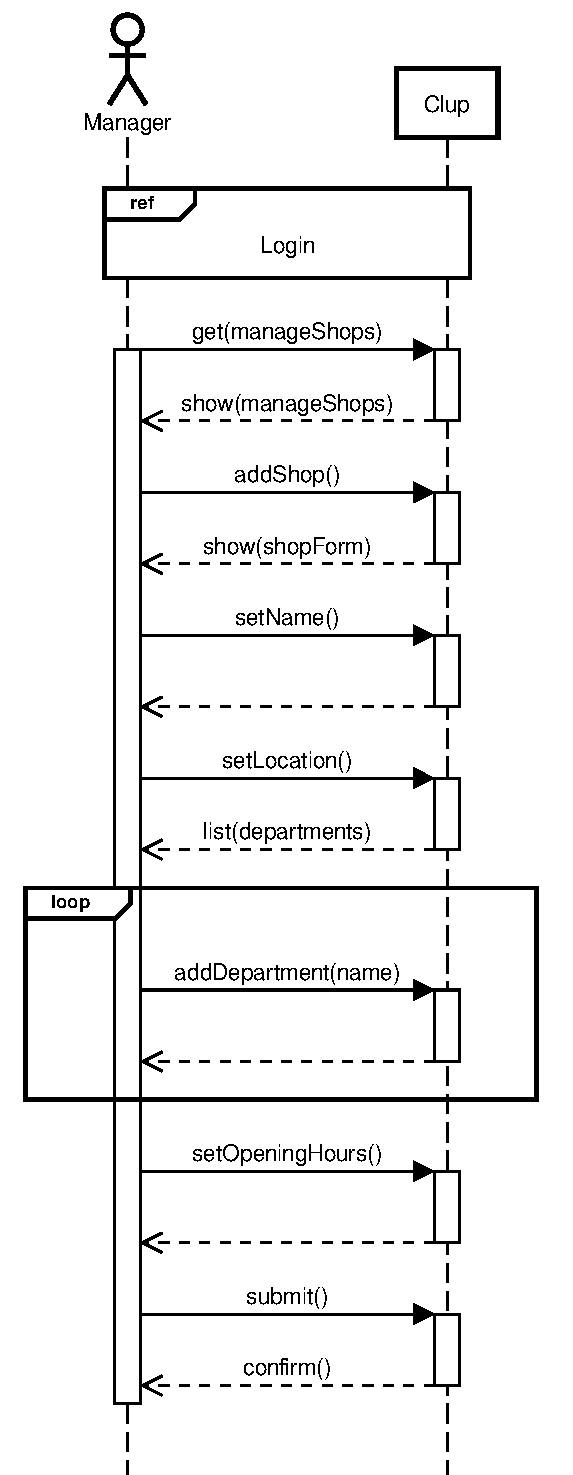
\includegraphics[scale=0.9]{Images/Sequence/add-shop_sequence_straight.pdf}
    \caption{Sequence Diagram for the creation of a Shop}
\end{figure}
\begin{figure}[H]
    \centering
    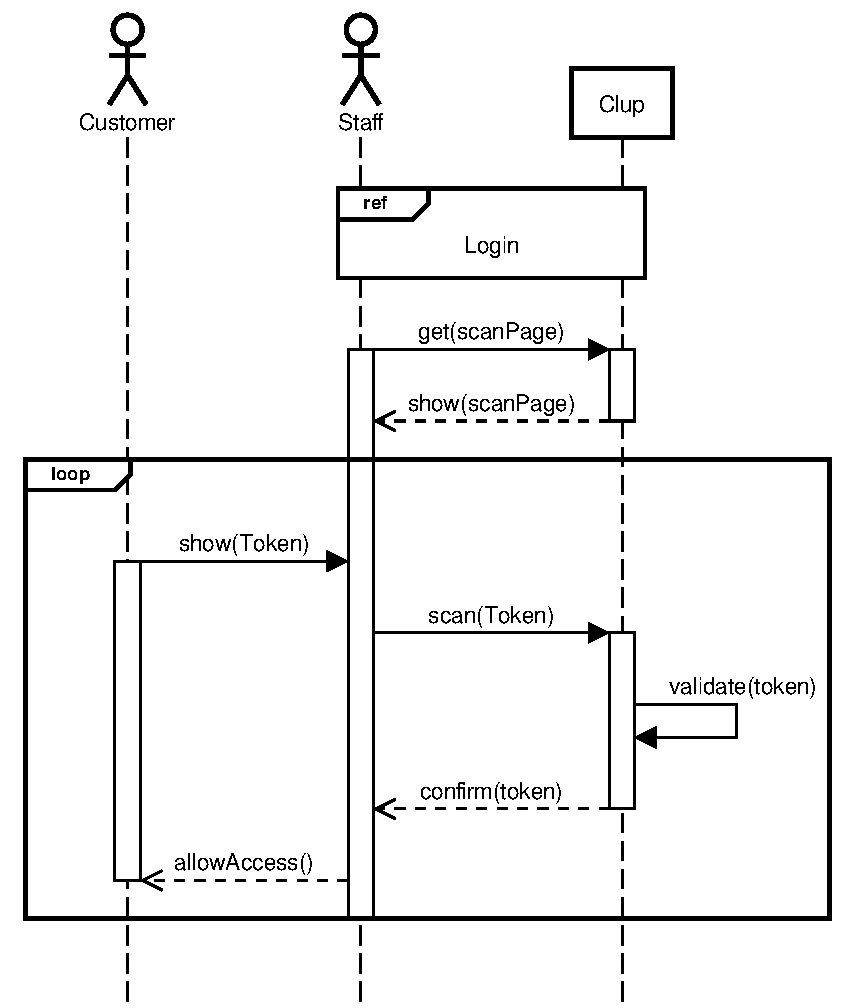
\includegraphics[scale=0.9]{Images/Sequence/scan-token_sequence_straight.pdf}
    \caption{Sequence Diagram for the scan of a valid Token}
\end{figure}
\begin{figure}[H]
    \centering
    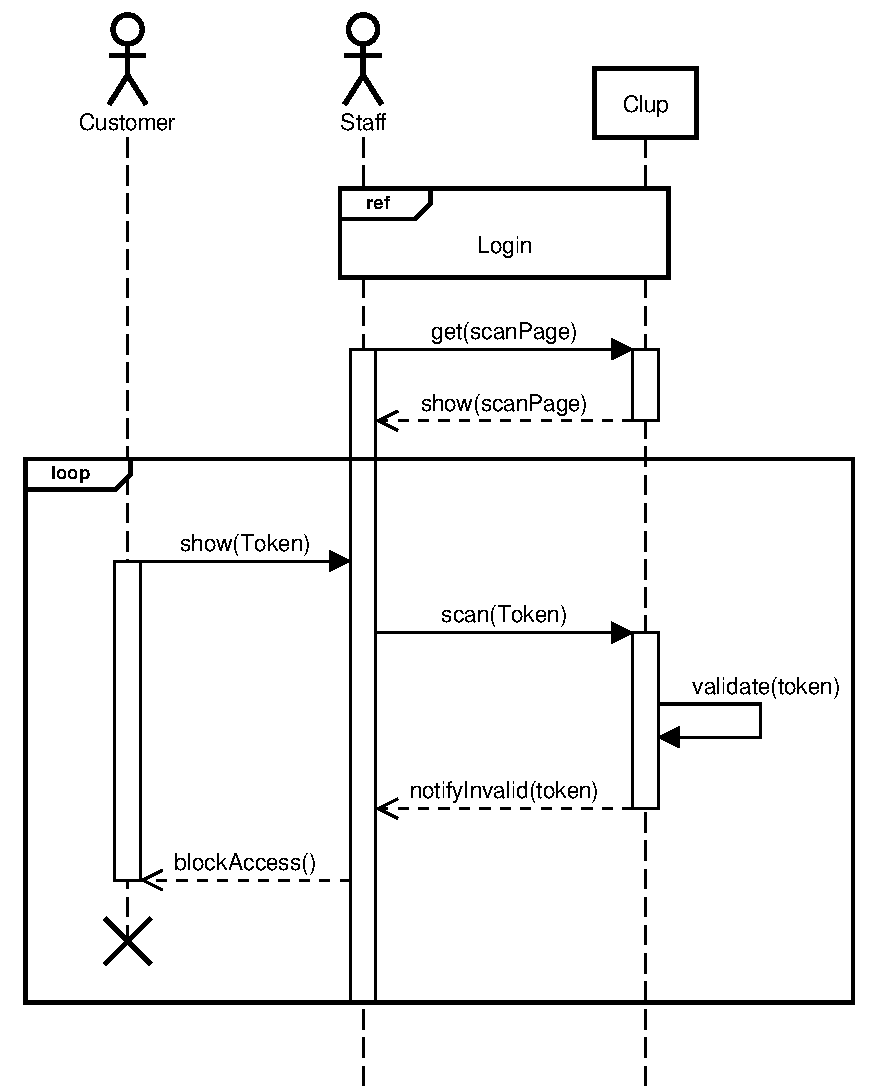
\includegraphics[scale=0.9]{Images/Sequence/failedscan-token_sequence_straight.pdf}
    \caption{Sequence Diagram for the scan of an invalid Token}
\end{figure}
\begin{figure}[H]
    \centering
    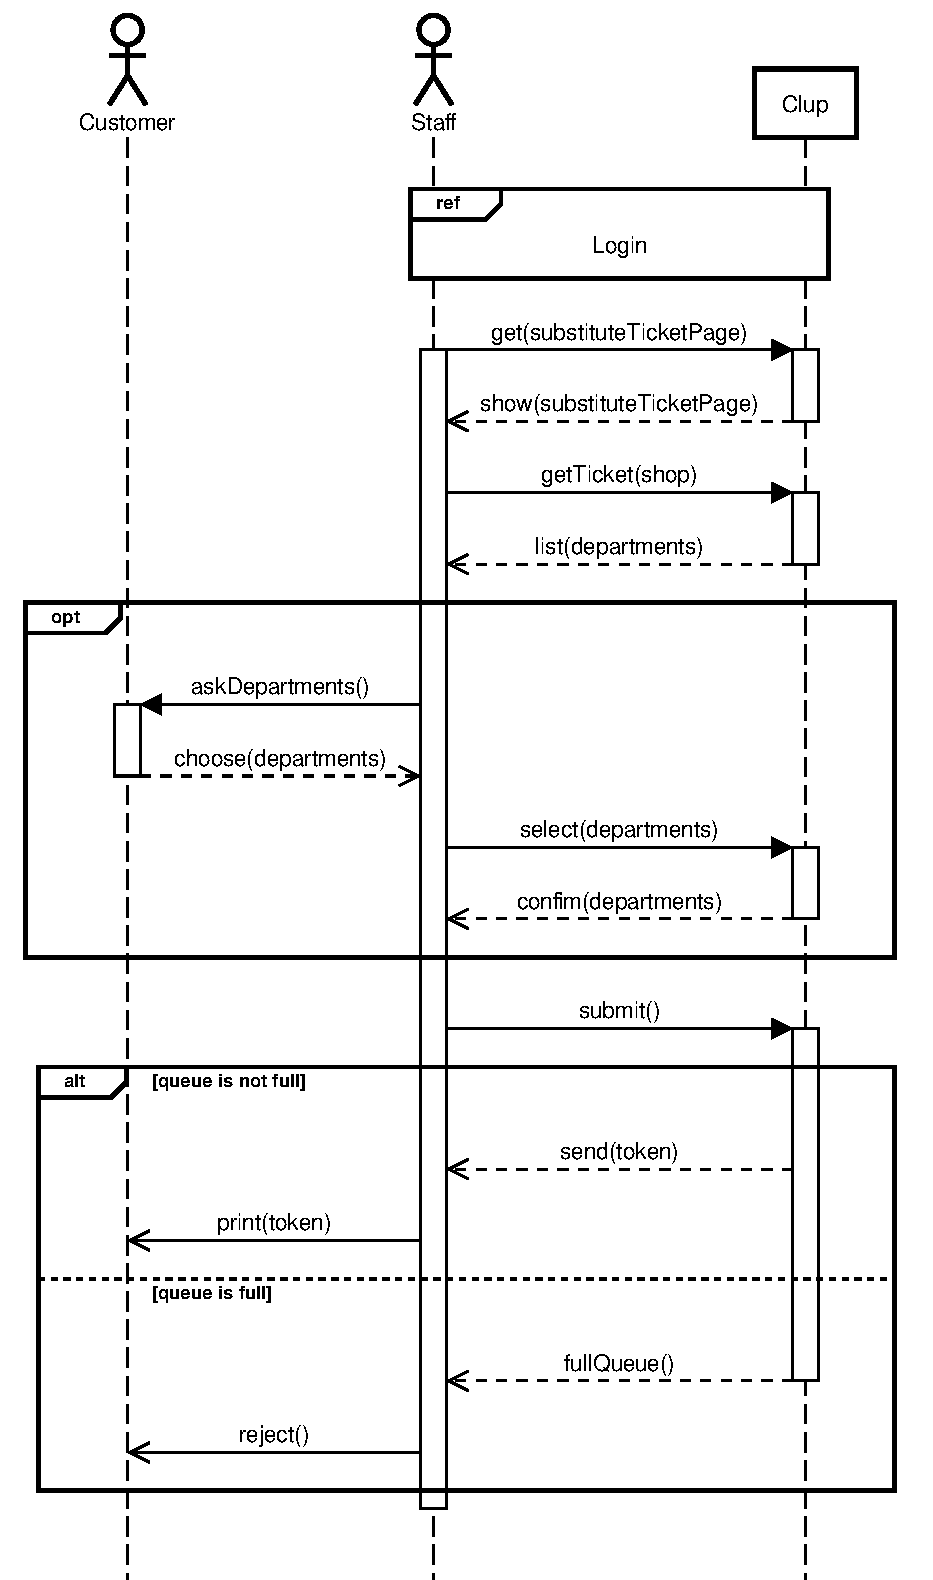
\includegraphics[scale=0.9]{Images/Sequence/substitute-ticket_sequence_straight.pdf}
    \caption{Sequence Diagram for the generation of a Substitute Token}
\end{figure}

\subsection{Performance Requirements}
\begin{itemize}
    \item Validating a token must be done as soon as possible and in no more than 5 seconds from when the token was acquired by the staff. This is required to achieve sufficient throughput and prevent queues from forming at the entrance.
    \item When obtaining a token the customer shall receive a response from the server within 15 seconds, since in this case time is not critical.
    \item Tokens shall be added to the system as soon as possible within 30 seconds.
\end{itemize}
\subsection{Design constraints}
\subsubsection{Standards compliance}
The web server shall comply to the HTTPS\footnote{\href{https://tools.ietf.org/html/rfc2818}{RFC2818: HTTP Over TLS}} protocol and target the HTTP/2\footnote{\href{https://tools.ietf.org/html/rfc7540}{RFC7540: Hypertext Transfer Protocol Version 2 (HTTP/2)}} standard for communication and the HTML5\footnote{\href{https://www.w3.org/TR/2017/REC-html52-20171214/}{HTML 5.2 W3C Recommendation, 14 December 2017}} standard for web pages.

\subsubsection{Hardware limitations}
Running the app requires a smartphone that supports one of the modern web browser engines; older cellphones whose official support has been discontinued shall not be supported.
To allow the validation of tickets by the Third Party Staff, the device should also be equipped with a camera of any resolution above 8 Megapixel.
%\subsubsection{Other constraints}

\subsection{Software System Attributes}
\subsubsection{Reliability}
\textit{CLup} should be available 24/7 in order to allow Customers to generate Tokens at any time of the day. Downtime due to maintenance shall be during the night and no longer than 2 hours, furthermore, customers and third parties shall be notified at least 3 days prior the scheduled downtime.
\subsubsection{Availability}
\emph{CLup} does not have a critical nature, however any downtime could cause serious problems to the management of the entrances to Shops. Hence, 99\% availability during daytime is required for \emph{CLup} to be effective. At night time, the availability requirement can be relaxed to 95\%.
\subsubsection{Security}
All communication should be over HTTPS protocol to provide privacy, data integrity and authentication.
Customer passwords shall be stored in a salted hash format.
The system should keep thorough logs of the activity of logged in customers and of login attempts. The registration and login procedure should not disclose informations about existing customers and repeated login attempts shall be limited.
Further details about the cryptographic functions and protocols employed will be discussed in the Design Document.
\subsubsection{Maintainability}
The system components shall be realized with high modularity and orthogonality between modules. This allows modifications to the code to be localized and leave the other components unaffected, minimizing the time required to fix problems with the system.
The backend system shall be able to run a test instance of the service that can be used by developers to test out features before deploying them to the main instance.
\subsubsection{Portability}
\textit{Clup} should be easily deployable on a dedicated machine, on a virtual private server or on a cloud hosting service. The server should be able to run both natively and in a containerized environment for maximum portability.


%------------------------------------------------------------------------------------------------------------------------------------------------
\clearpage
{\color{Blue}{\section{Formal Analysis Using Alloy}}}
\label{sect:alloy}
\subsection{Introduction}
This chapter presents a formal analysis of the application. Since the application domain is time dependent at its core, we decided to model the evolution of the system over time, with focus on the entrances to the Shops. The model focuses on Customers, Tickets and Bookings: the Staff can be seen as an intermediary and moderator between the Customers and the system, therefore, by assuming that the Staff will follow the rules, we can simplify the model for clarity and ease of comprehension.
The scenario being analyzed starts from a state in which Customers already have acquired the tokens and enter the Shops. The queue uses strict constraints, by allowing only the first in queue to enter the Shop. In practice, the constraint can be relaxed to increase throughput if needed. 
In particular, the model checks the following properties:
\begin{itemize}
    \item No department in a Shop exceeds its occupancy limits
    \item Customers cannot enter a Shop without a valid Token
    \item Customers can use a Booking to enter a Shop only at the time specified
    \item Customers cannot cut the waiting line for a Shop
    \item The same Token cannot be used for multiple visits
\end{itemize}
\subsection{Alloy code}
\subsubsection{Model description}
The first section describes the signatures of the objects which are relevant for the formal analysis and their representation invariants.
\lstinputlisting[language=alloy,firstline=1,lastline=68]{alloy/main.als}
\subsubsection{Dynamic properties}
This section describes the rules that guarantee the correct evolution of the system over time. In particular, the \texttt{Trace} fact rules the transition from an instant to the next for Customers and for the Waiting List. 
\lstinputlisting[language=alloy,firstline=72,lastline=127]{alloy/main.als}
\subsubsection{Assertions}
This section lists some of the property that will be guaranteed \emph{if} the invariants described in the previous sections hold. The The result of the evaluation of these assertions will be presented in the next section.
\lstinputlisting[language=alloy,firstline=131,lastline=211]{alloy/main.als}
\subsubsection{Execution results}
This section shows the experimental result of the formal analysis 
\lstinputlisting[language=alloy,firstline=215]{alloy/main.als}

\pagebreak
The following figures show the evolution of a particular instance of the enterAndExit predicate, for 5 consecutive Time instants. A visiting Customer is pointed out by a \emph{visiting} connection to one of the Visit elements, which, in turn, is connected to a set of Department nodes of the same Shop.
\begin{figure}[H]
    \centering
    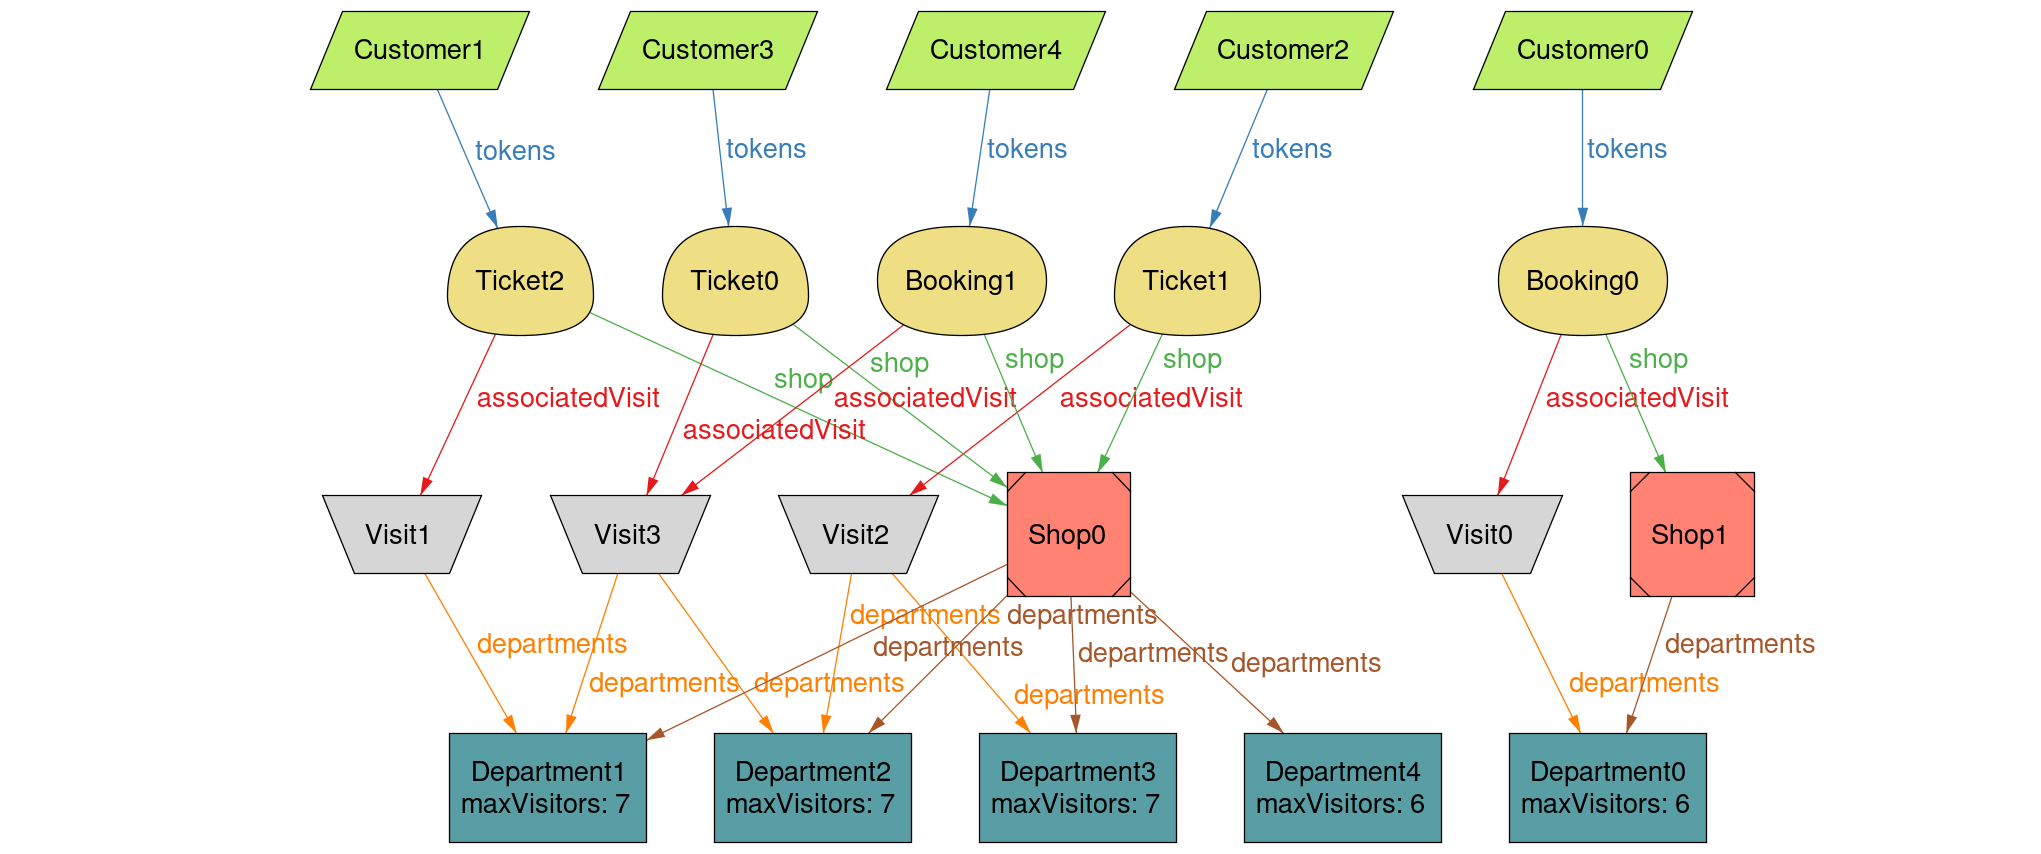
\includegraphics[height=0.25\textheight]{Images/Alloy/5Customers_v1_t0.png}
    \caption{Run for Time 0. This is the initial state.}
\end{figure}
\begin{figure}[H]
    \centering
    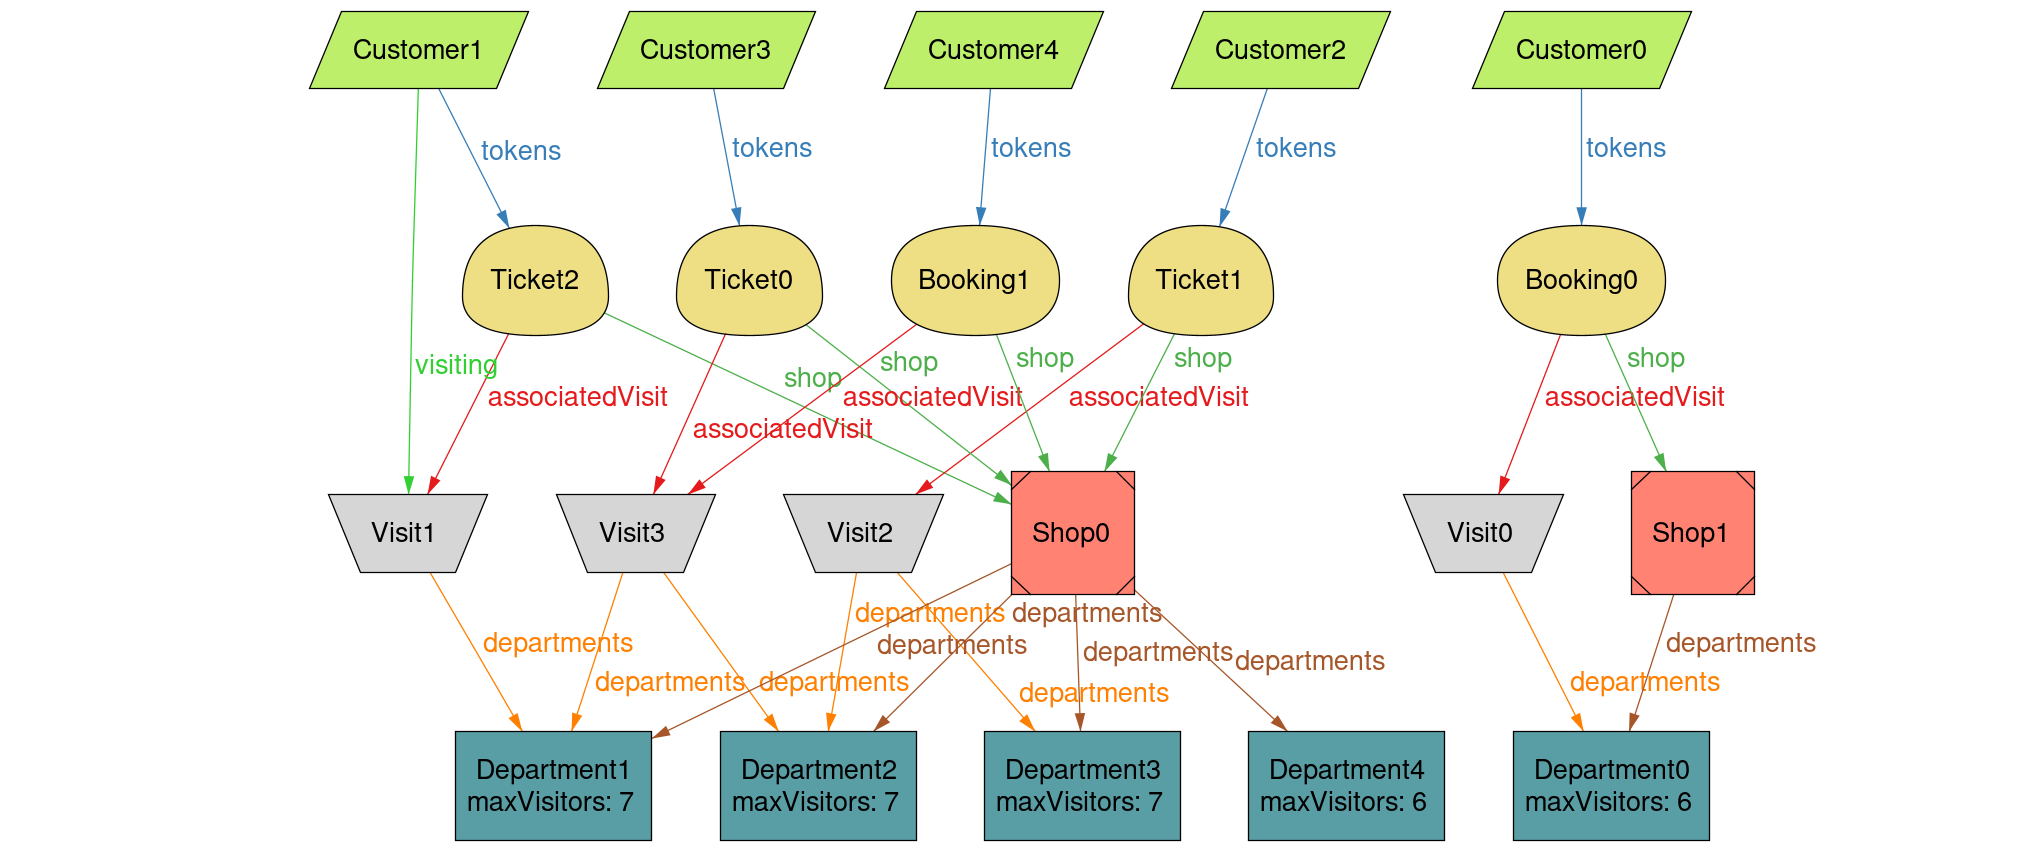
\includegraphics[height=0.25\textheight]{Images/Alloy/5Customers_v1_t1.png}
    \caption{Run for Time 1. \emph{Customer1} has used his Ticket to enter \emph{Shop0}.}
\end{figure}
\begin{figure}[H]
    \centering
    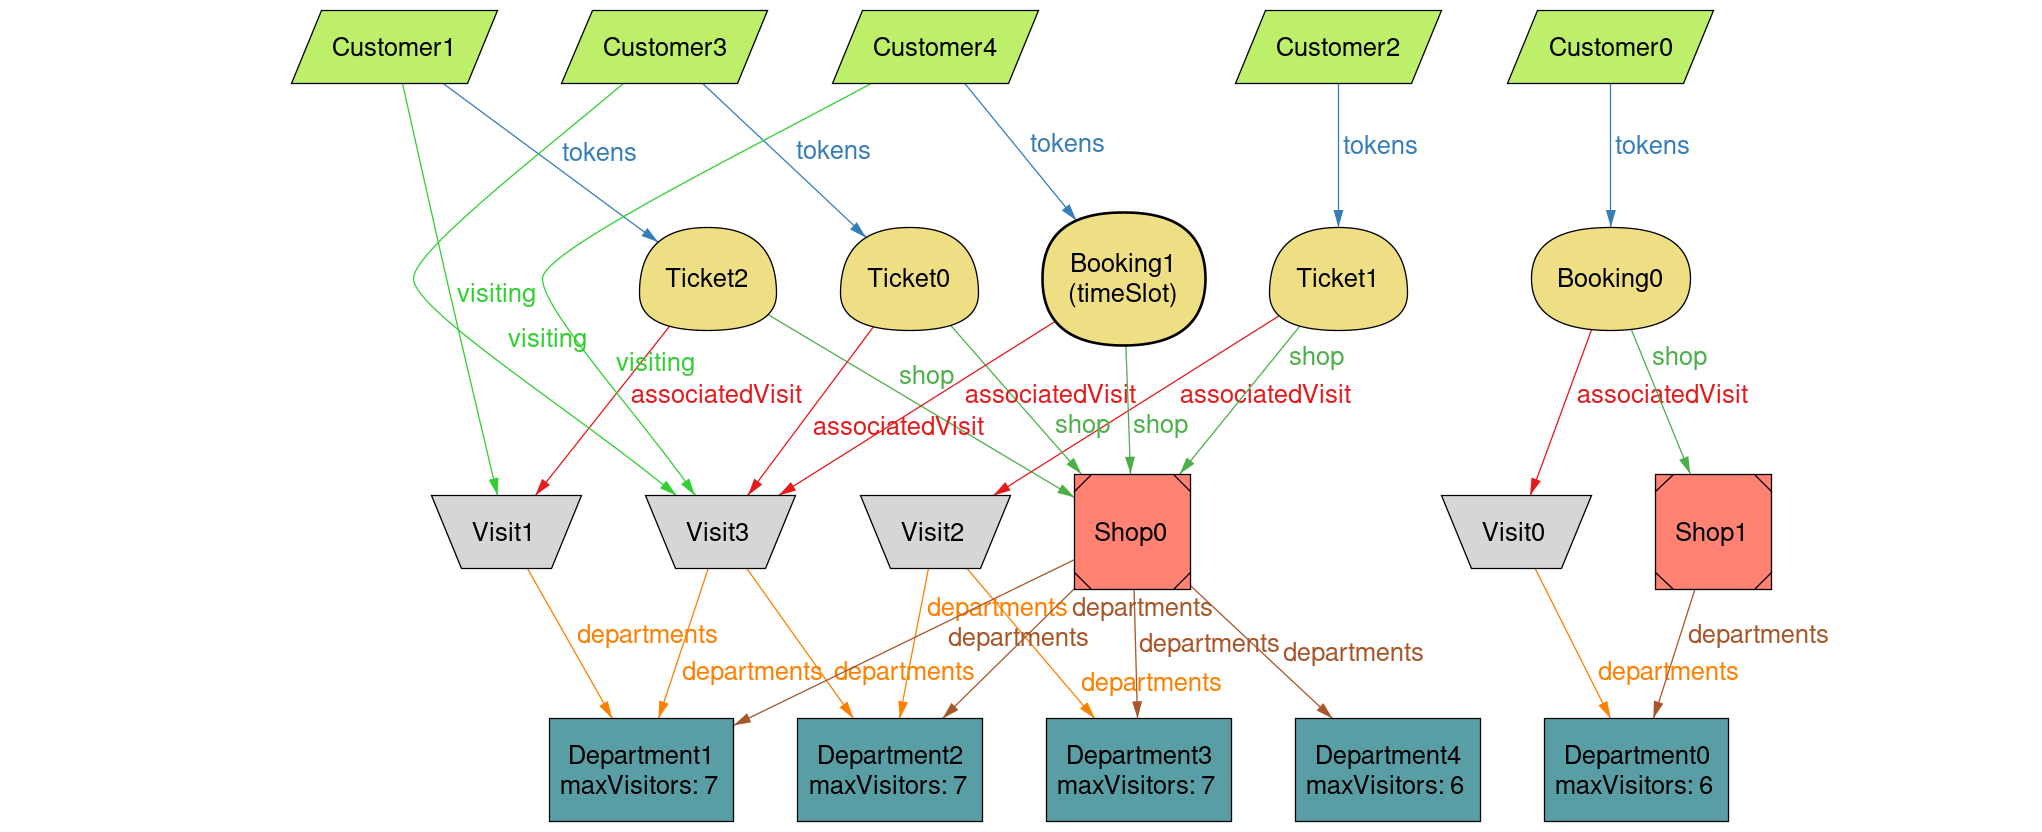
\includegraphics[height=0.25\textheight]{Images/Alloy/5Customers_v1_t2.png}
    \caption{Run for Time 2. \emph{Customer3} and \emph{4} enter the same shop with a Ticket and a Booking respectively.}
\end{figure}
\begin{figure}[H]
    \centering
    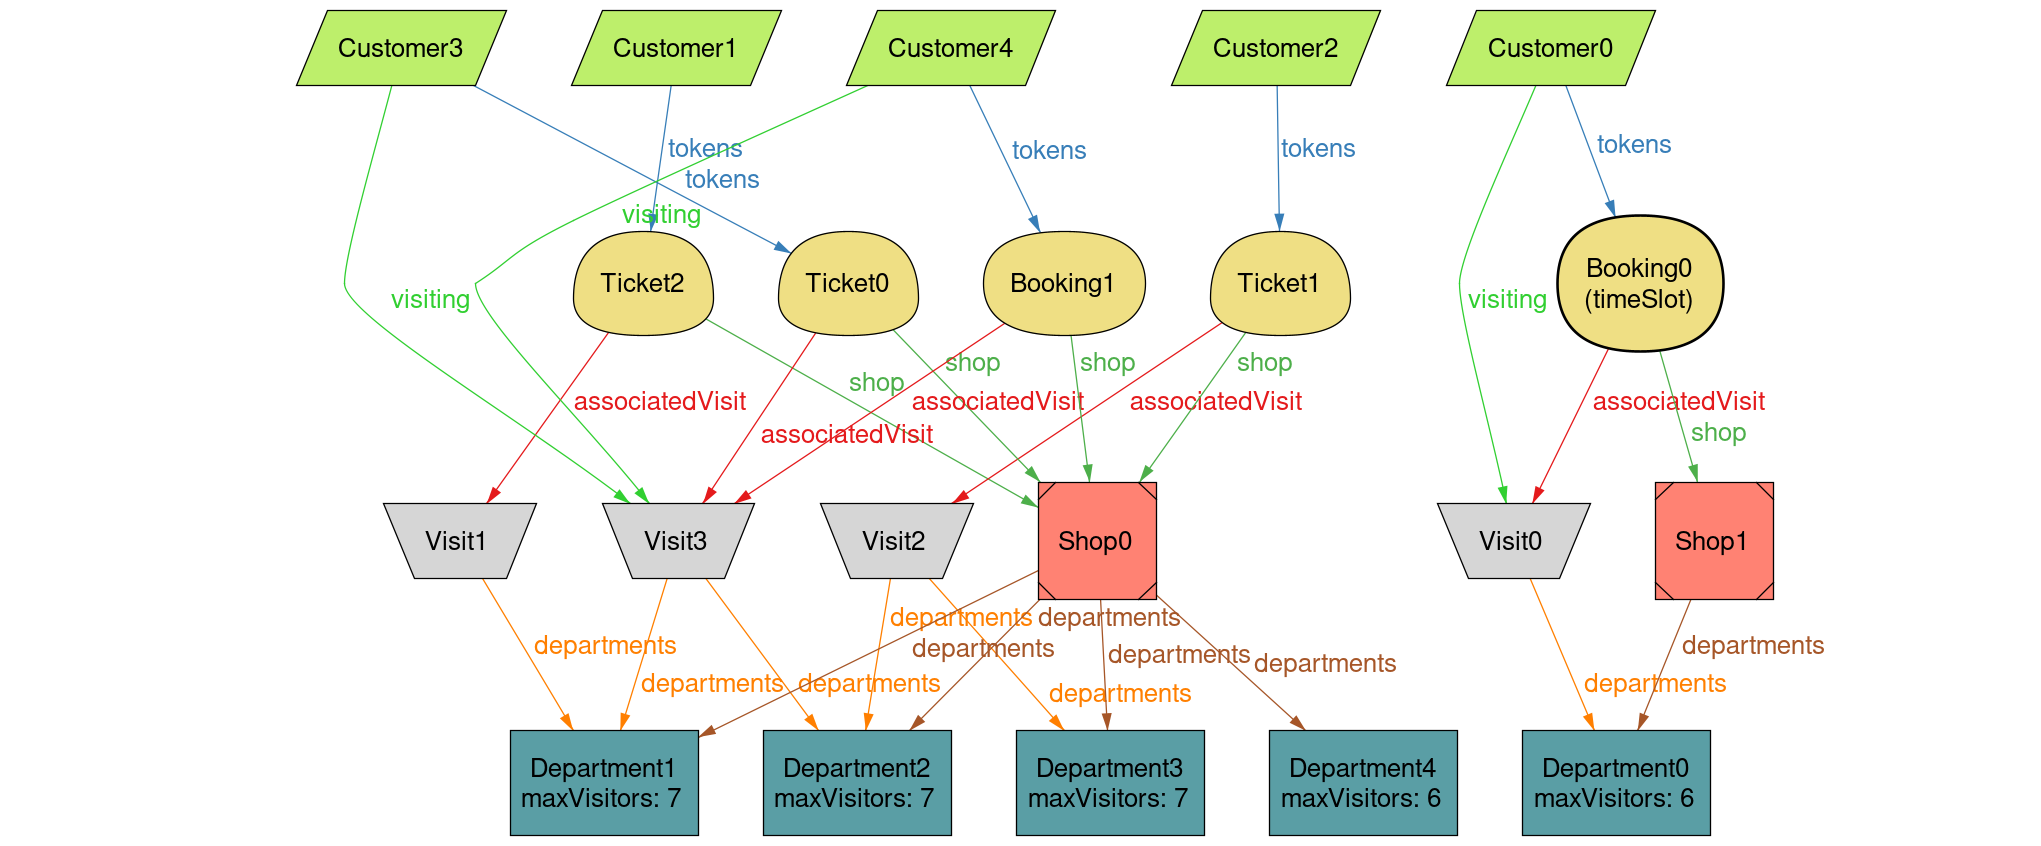
\includegraphics[height=0.25\textheight]{Images/Alloy/5Customers_v1_t3.png}
    \caption{Run for Time 3. \emph{Customer1} correctly exits \emph{Shop0}, while \emph{Customer0} makes use of a Booking for \emph{Shop1}}
\end{figure}
\begin{figure}[H]
    \centering
    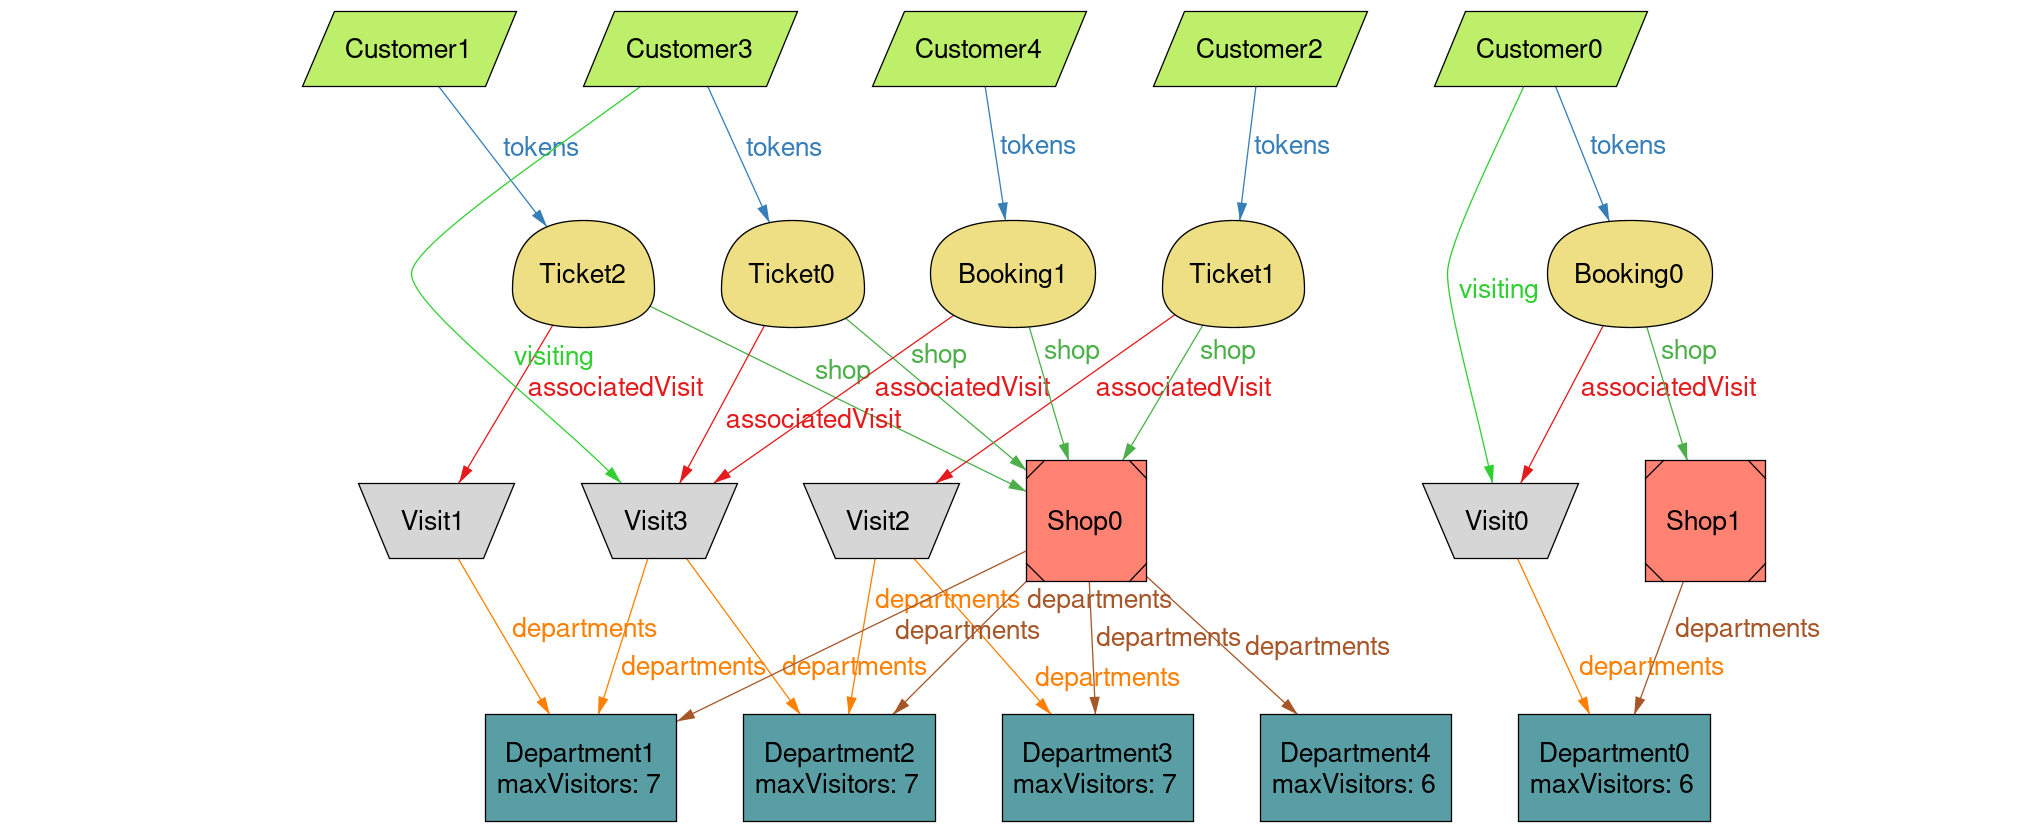
\includegraphics[height=0.25\textheight]{Images/Alloy/5Customers_v1_t4.png}
    \caption{Run for Time 4. \emph{Customer4} exits as well.}
\end{figure}

\pagebreak
Figure \ref{fig:waitinglistnode1} and \ref{fig:waitinglistnode2} provide a more detailed view of the same instance, displaying the working principle of the waiting List. Each WaitingListNode represents a single Customer in line, with their Ticket. In the first figure, set at Time 0, we see that \emph{Customer1} has the Ticket corresponding to the first WaitingListNode for \emph{Shop0}, pointed by the \emph{queue} attribute, thus he is allowed to enter at the next time frame.
Indeed, in the second figure, set at Time 1, a new \emph{visiting} connection between \emph{Customer1} and \emph{Visit1} is spawned, which means that the Customer is visiting \emph{Department1} of \emph{Shop0}. The \emph{queue} attribute of the Shop has also been moved forward to a new WaitingListNode, as expected.
\begin{figure}[H]
    \centering
    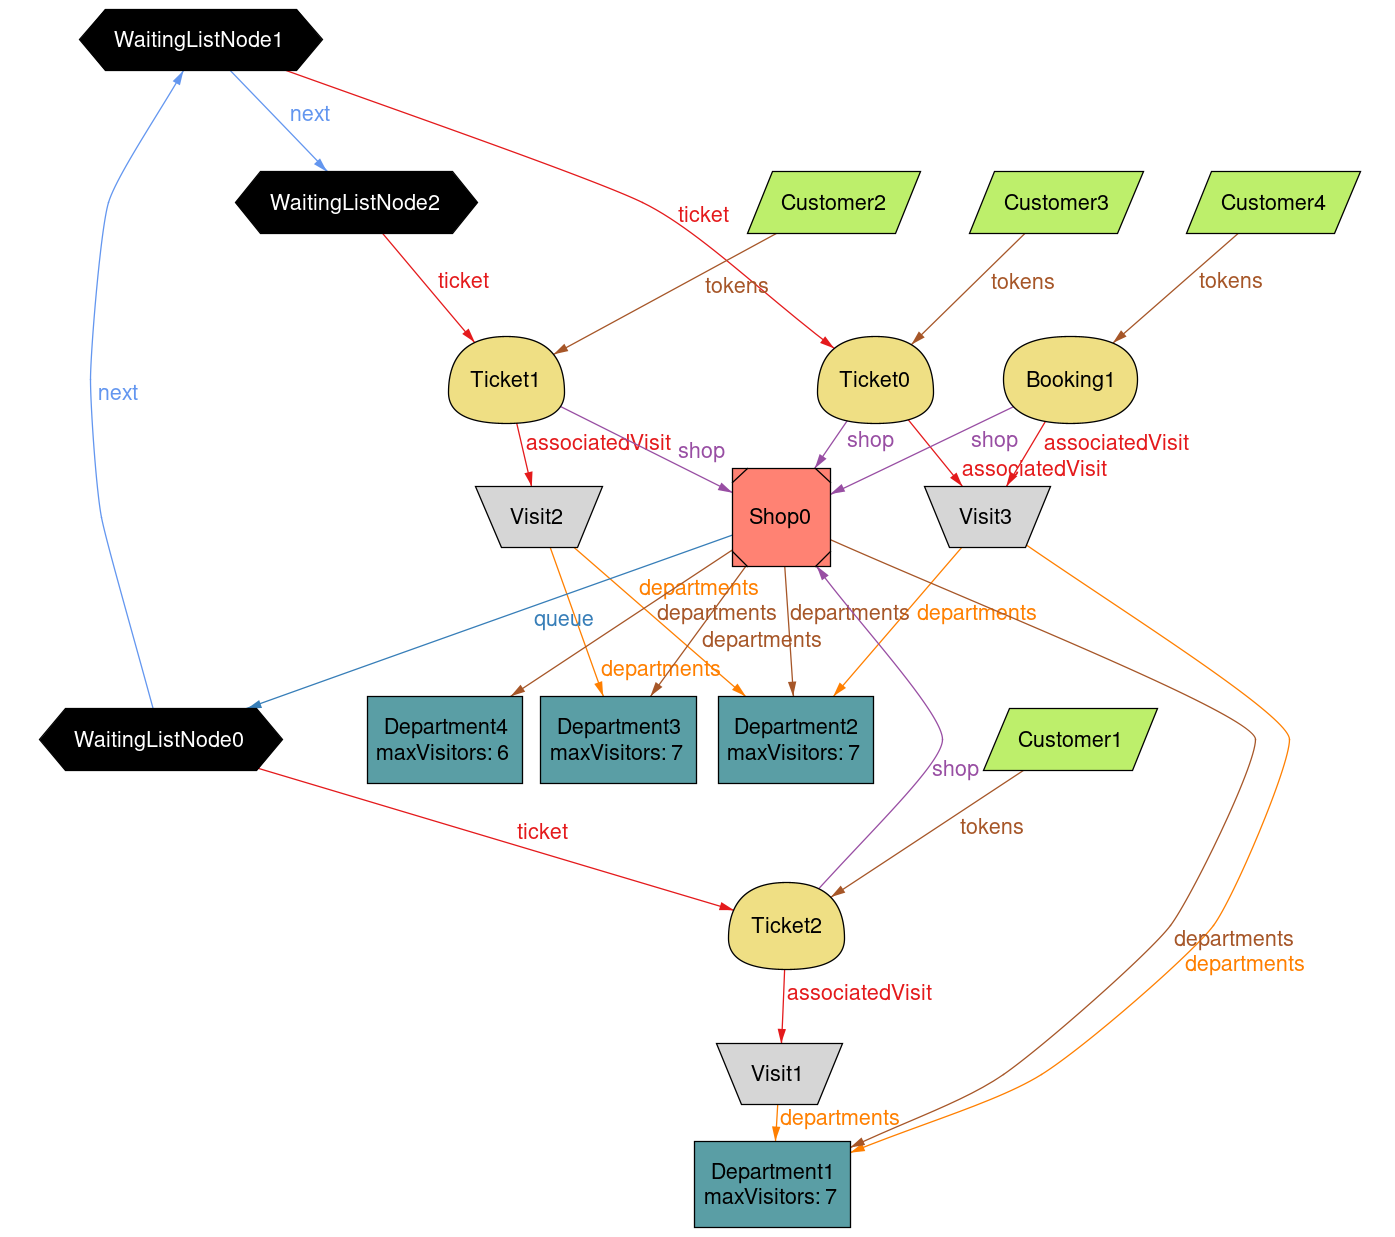
\includegraphics[width=\textwidth]{Images/Alloy/5Customers_v1_t0_detail_crop.png}
    \caption{The same instance at Time 0, with WaitingListNode elements shown}
    \label{fig:waitinglistnode1}
\end{figure}
\begin{figure}[H]
    \centering
    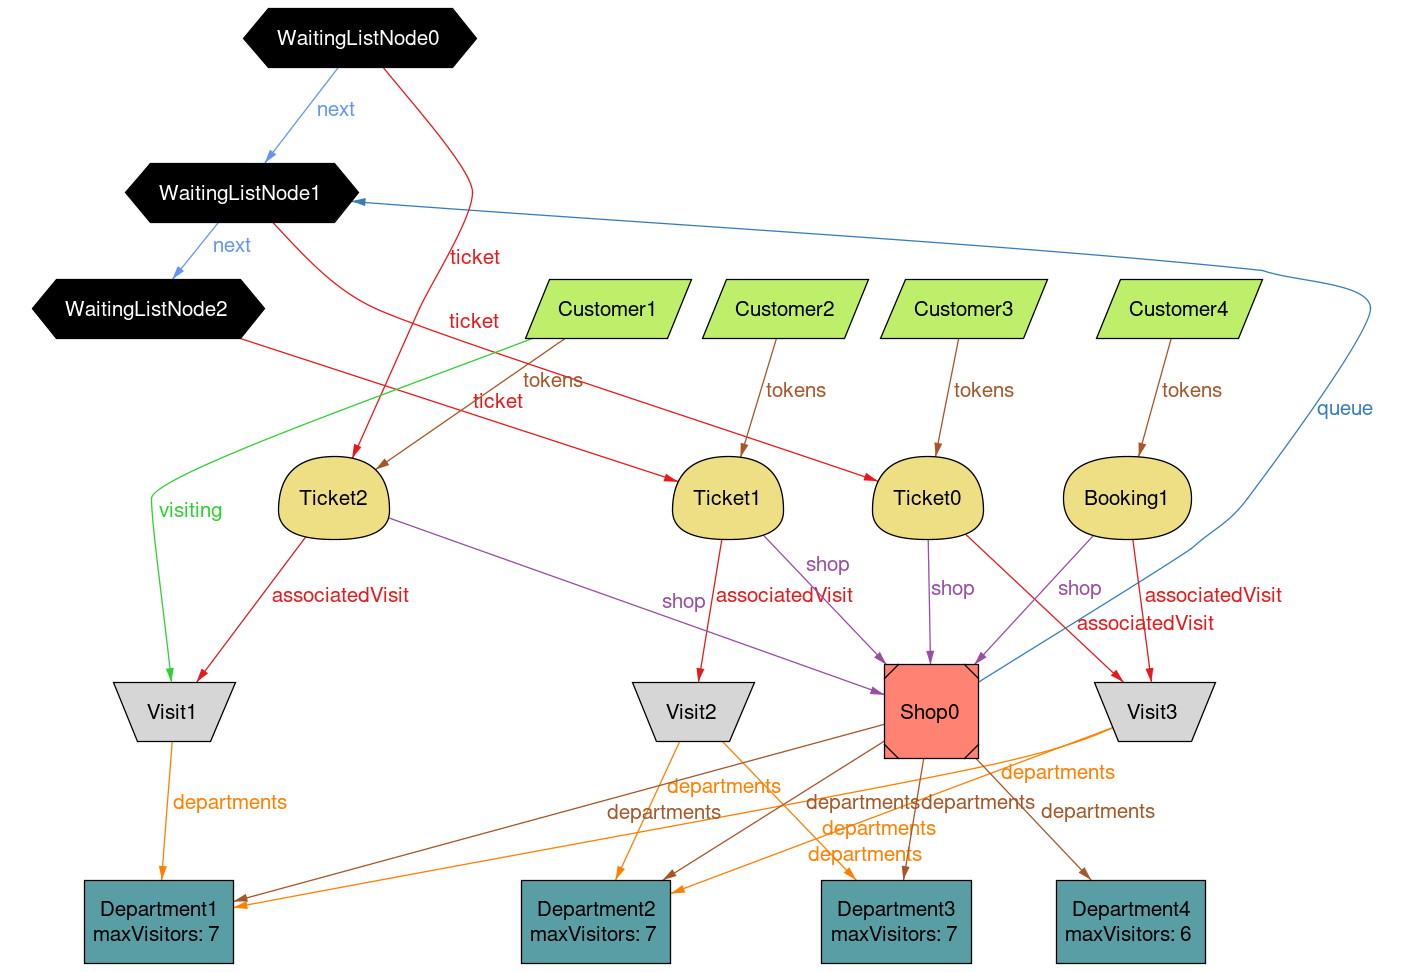
\includegraphics[width=\textwidth]{Images/Alloy/5Customers_v1_t1_detail_crop.png}
    \caption{The evolution of the instance at Time 1}
    \label{fig:waitinglistnode2}
\end{figure}

%------------------------------------------------------------------------------------------------------------------------------------------------
\clearpage
{\color{Blue}{\section{Effort Spent}}}
\label{sect:effort}

\begin{table}[H]
    \centering
    \begin{tabular}{|l|l|l|}
        \multicolumn{3}{c}{\textbf{Luca De Martini}}                   \\
        \hline
        \textbf{Date} & \textbf{Hours} & \textbf{Description}          \\\hline
        2020-12-28    & 3h             & First Meeting       \\\hline
        2020-12-29    & 3h             & Introduction       \\\hline
        2020-12-30    & 4h             & API       \\\hline
        2021-1-1    & 2h             & API       \\\hline
        2021-1-2    & 2h             & API \& Deployment       \\\hline
        2021-1-3    & 2h             & Architecture       \\\hline
        2021-1-4    & 3h             & Review \& API       \\\hline
        2021-1-5    & 5h             & Review \& API       \\\hline
        2021-1-6    & 3h             & Implementation Plan       \\\hline
    \end{tabular}
\end{table}
\begin{table}[H]
    \centering
    \begin{tabular}{|l|l|l|}
        \multicolumn{3}{c}{\textbf{Alessandro Duico}}                      \\
        \hline
        \textbf{Date} & \textbf{Hours} & \textbf{Description}              \\\hline
        2020-12-28    & 3h             & First Meeting           \\\hline
        2020-12-29    & 3h             & Introduction       \\\hline
        2020-12-30    & 3h             & Component view     \\\hline
        2020-12-1     & 4h             & Deployment diagram \\\hline
        2021-1-2     & 1h             & Runtime View   \\\hline
        2021-1-4     & 3h             & Runtime View   \\\hline
        2021-1-5     & 3h             & Review \\\hline
    \end{tabular}
\end{table}



%------------------------------------------------------------------------------------------------------------------------------------------------
\clearpage
\addcontentsline{toc}{section}{References}
\bibliographystyle{plain}
\bibliography{main}
%------------------------------------------------------------------------------------------------------------------------------------------------




\end{document}
